\documentclass[a4paper]{book}
\usepackage{a4wide}
\usepackage{makeidx}
\usepackage{graphicx}
\usepackage{multicol}
\usepackage{float}
\usepackage{listings}
\usepackage{color}
\usepackage{textcomp}
\usepackage{alltt}
\usepackage{times}
\usepackage{ifpdf}
\ifpdf
\usepackage[pdftex,
            pagebackref=true,
            colorlinks=true,
            linkcolor=blue,
            unicode
           ]{hyperref}
\else
\usepackage[ps2pdf,
            pagebackref=true,
            colorlinks=true,
            linkcolor=blue,
            unicode
           ]{hyperref}
\usepackage{pspicture}
\fi
\usepackage[utf8]{inputenc}
\usepackage{doxygen}
\lstset{language=C++,inputencoding=utf8,basicstyle=\footnotesize,breaklines=true,breakatwhitespace=true,tabsize=8,numbers=left }
\makeindex
\setcounter{tocdepth}{3}
\renewcommand{\footrulewidth}{0.4pt}
\begin{document}
\hypersetup{pageanchor=false}
\begin{titlepage}
\vspace*{7cm}
\begin{center}
{\Large Sigma \\[1ex]\large 1.0 }\\
\vspace*{1cm}
{\large Generated by Doxygen 1.6.1}\\
\vspace*{0.5cm}
{\small Fri Jun 20 10:59:52 2014}\\
\end{center}
\end{titlepage}
\clearemptydoublepage
\pagenumbering{roman}
\tableofcontents
\clearemptydoublepage
\pagenumbering{arabic}
\hypersetup{pageanchor=true}
\chapter{Class Index}
\section{Class Hierarchy}
This inheritance list is sorted roughly, but not completely, alphabetically:\begin{DoxyCompactList}
\item \contentsline{section}{Cluster}{\pageref{classCluster}}{}
\item \contentsline{section}{ClusterGraph}{\pageref{classClusterGraph}}{}
\item \contentsline{section}{Contig}{\pageref{classContig}}{}
\item \contentsline{section}{ContigIO}{\pageref{classContigIO}}{}
\item \contentsline{section}{ContigReader}{\pageref{classContigReader}}{}
\begin{DoxyCompactList}
\item \contentsline{section}{SOAPdenovoReader}{\pageref{classSOAPdenovoReader}}{}
\item \contentsline{section}{VelvetReader}{\pageref{classVelvetReader}}{}
\end{DoxyCompactList}
\item \contentsline{section}{Edge}{\pageref{classEdge}}{}
\item \contentsline{section}{EdgeComparator}{\pageref{classEdgeComparator}}{}
\item \contentsline{section}{EdgeHash}{\pageref{classEdgeHash}}{}
\item \contentsline{section}{EdgeReader}{\pageref{classEdgeReader}}{}
\begin{DoxyCompactList}
\item \contentsline{section}{OperaBundleReader}{\pageref{classOperaBundleReader}}{}
\end{DoxyCompactList}
\item \contentsline{section}{MappingReader}{\pageref{classMappingReader}}{}
\begin{DoxyCompactList}
\item \contentsline{section}{SAMReader}{\pageref{classSAMReader}}{}
\end{DoxyCompactList}
\item \contentsline{section}{ProbabilityDistribution}{\pageref{classProbabilityDistribution}}{}
\begin{DoxyCompactList}
\item \contentsline{section}{NegativeBinomialDistribution}{\pageref{classNegativeBinomialDistribution}}{}
\item \contentsline{section}{PoissonDistribution}{\pageref{classPoissonDistribution}}{}
\end{DoxyCompactList}
\item \contentsline{section}{Sigma}{\pageref{classSigma}}{}
\end{DoxyCompactList}

\chapter{Class Index}
\section{Class List}
Here are the classes, structs, unions and interfaces with brief descriptions:\begin{DoxyCompactList}
\item\contentsline{section}{\hyperlink{classCluster}{Cluster} (A class for representing clusters in hierarchical clustering trees )}{\pageref{classCluster}}{}
\item\contentsline{section}{\hyperlink{classClusterGraph}{ClusterGraph} (A class for representing a graph of hierarchical clustering trees )}{\pageref{classClusterGraph}}{}
\item\contentsline{section}{\hyperlink{classContig}{Contig} (A class for representing contigs in the assembly graph )}{\pageref{classContig}}{}
\item\contentsline{section}{\hyperlink{classContigIO}{ContigIO} (Class containing internal contigs IO functions )}{\pageref{classContigIO}}{}
\item\contentsline{section}{\hyperlink{classContigReader}{ContigReader} (An interface for contigs file readers )}{\pageref{classContigReader}}{}
\item\contentsline{section}{\hyperlink{classEdge}{Edge} (A class for representing scaffold edges in the assembly graph )}{\pageref{classEdge}}{}
\item\contentsline{section}{\hyperlink{classEdgeComparator}{EdgeComparator} (Function object class for less-\/than inequality comparison of \hyperlink{classEdge}{Edge} objects )}{\pageref{classEdgeComparator}}{}
\item\contentsline{section}{\hyperlink{classEdgeHash}{EdgeHash} (Function object class for computing hash values for \hyperlink{classEdge}{Edge} objects )}{\pageref{classEdgeHash}}{}
\item\contentsline{section}{\hyperlink{classEdgeReader}{EdgeReader} (An interface for edges file readers )}{\pageref{classEdgeReader}}{}
\item\contentsline{section}{\hyperlink{classMappingReader}{MappingReader} (An interface for mapping file readers )}{\pageref{classMappingReader}}{}
\item\contentsline{section}{\hyperlink{classNegativeBinomialDistribution}{NegativeBinomialDistribution} (An implementation of negative binomial probability distribution )}{\pageref{classNegativeBinomialDistribution}}{}
\item\contentsline{section}{\hyperlink{classOperaBundleReader}{OperaBundleReader} (Opera edges file reader )}{\pageref{classOperaBundleReader}}{}
\item\contentsline{section}{\hyperlink{classPoissonDistribution}{PoissonDistribution} (An implementation of Poisson probability distribution )}{\pageref{classPoissonDistribution}}{}
\item\contentsline{section}{\hyperlink{classProbabilityDistribution}{ProbabilityDistribution} (An interface for probability distributions )}{\pageref{classProbabilityDistribution}}{}
\item\contentsline{section}{\hyperlink{classSAMReader}{SAMReader} (SAM mapping file reader )}{\pageref{classSAMReader}}{}
\item\contentsline{section}{\hyperlink{classSigma}{Sigma} (Main configuration class )}{\pageref{classSigma}}{}
\item\contentsline{section}{\hyperlink{classSOAPdenovoReader}{SOAPdenovoReader} (SOAPdenovo contigs file reader )}{\pageref{classSOAPdenovoReader}}{}
\item\contentsline{section}{\hyperlink{classVelvetReader}{VelvetReader} (Velvet contigs file reader )}{\pageref{classVelvetReader}}{}
\end{DoxyCompactList}

\chapter{File Index}
\section{File List}
Here is a list of all files with brief descriptions:\begin{DoxyCompactList}
\item\contentsline{section}{/mnt/ScratchPool/bertrandd/OPERA\_\-MS/OperaMS2.0/SIGMA++/1.4/\hyperlink{cluster_8cpp}{cluster.cpp} }{\pageref{cluster_8cpp}}{}
\item\contentsline{section}{/mnt/ScratchPool/bertrandd/OPERA\_\-MS/OperaMS2.0/SIGMA++/1.4/\hyperlink{cluster_8h}{cluster.h} }{\pageref{cluster_8h}}{}
\item\contentsline{section}{/mnt/ScratchPool/bertrandd/OPERA\_\-MS/OperaMS2.0/SIGMA++/1.4/\hyperlink{cluster__graph_8cpp}{cluster\_\-graph.cpp} }{\pageref{cluster__graph_8cpp}}{}
\item\contentsline{section}{/mnt/ScratchPool/bertrandd/OPERA\_\-MS/OperaMS2.0/SIGMA++/1.4/\hyperlink{cluster__graph_8h}{cluster\_\-graph.h} }{\pageref{cluster__graph_8h}}{}
\item\contentsline{section}{/mnt/ScratchPool/bertrandd/OPERA\_\-MS/OperaMS2.0/SIGMA++/1.4/\hyperlink{contig_8cpp}{contig.cpp} }{\pageref{contig_8cpp}}{}
\item\contentsline{section}{/mnt/ScratchPool/bertrandd/OPERA\_\-MS/OperaMS2.0/SIGMA++/1.4/\hyperlink{contig_8h}{contig.h} }{\pageref{contig_8h}}{}
\item\contentsline{section}{/mnt/ScratchPool/bertrandd/OPERA\_\-MS/OperaMS2.0/SIGMA++/1.4/\hyperlink{contig__reader_8cpp}{contig\_\-reader.cpp} }{\pageref{contig__reader_8cpp}}{}
\item\contentsline{section}{/mnt/ScratchPool/bertrandd/OPERA\_\-MS/OperaMS2.0/SIGMA++/1.4/\hyperlink{contig__reader_8h}{contig\_\-reader.h} }{\pageref{contig__reader_8h}}{}
\item\contentsline{section}{/mnt/ScratchPool/bertrandd/OPERA\_\-MS/OperaMS2.0/SIGMA++/1.4/\hyperlink{edge_8cpp}{edge.cpp} }{\pageref{edge_8cpp}}{}
\item\contentsline{section}{/mnt/ScratchPool/bertrandd/OPERA\_\-MS/OperaMS2.0/SIGMA++/1.4/\hyperlink{edge_8h}{edge.h} }{\pageref{edge_8h}}{}
\item\contentsline{section}{/mnt/ScratchPool/bertrandd/OPERA\_\-MS/OperaMS2.0/SIGMA++/1.4/\hyperlink{edge__reader_8cpp}{edge\_\-reader.cpp} }{\pageref{edge__reader_8cpp}}{}
\item\contentsline{section}{/mnt/ScratchPool/bertrandd/OPERA\_\-MS/OperaMS2.0/SIGMA++/1.4/\hyperlink{edge__reader_8h}{edge\_\-reader.h} }{\pageref{edge__reader_8h}}{}
\item\contentsline{section}{/mnt/ScratchPool/bertrandd/OPERA\_\-MS/OperaMS2.0/SIGMA++/1.4/\hyperlink{mapping__reader_8cpp}{mapping\_\-reader.cpp} }{\pageref{mapping__reader_8cpp}}{}
\item\contentsline{section}{/mnt/ScratchPool/bertrandd/OPERA\_\-MS/OperaMS2.0/SIGMA++/1.4/\hyperlink{mapping__reader_8h}{mapping\_\-reader.h} }{\pageref{mapping__reader_8h}}{}
\item\contentsline{section}{/mnt/ScratchPool/bertrandd/OPERA\_\-MS/OperaMS2.0/SIGMA++/1.4/\hyperlink{probability__distribution_8cpp}{probability\_\-distribution.cpp} }{\pageref{probability__distribution_8cpp}}{}
\item\contentsline{section}{/mnt/ScratchPool/bertrandd/OPERA\_\-MS/OperaMS2.0/SIGMA++/1.4/\hyperlink{probability__distribution_8h}{probability\_\-distribution.h} }{\pageref{probability__distribution_8h}}{}
\item\contentsline{section}{/mnt/ScratchPool/bertrandd/OPERA\_\-MS/OperaMS2.0/SIGMA++/1.4/\hyperlink{sigma_8cpp}{sigma.cpp} }{\pageref{sigma_8cpp}}{}
\item\contentsline{section}{/mnt/ScratchPool/bertrandd/OPERA\_\-MS/OperaMS2.0/SIGMA++/1.4/\hyperlink{sigma_8h}{sigma.h} }{\pageref{sigma_8h}}{}
\end{DoxyCompactList}

\chapter{Class Documentation}
\hypertarget{classCluster}{
\section{Cluster Class Reference}
\label{classCluster}\index{Cluster@{Cluster}}
}


A class for representing clusters in hierarchical clustering trees.  


{\ttfamily \#include $<$/mnt/ScratchPool/bertrandd/OPERA\_\-MS/OperaMS2.0/SIGMA++/1.4/cluster.h$>$}\subsection*{Public Member Functions}
\begin{DoxyCompactItemize}
\item 
\hyperlink{classCluster_a9f69adb0b24c9d63ef3a95902c07480d}{Cluster} (\hyperlink{classContig}{Contig} $\ast$contig)
\begin{DoxyCompactList}\small\item\em Constructs a singleton cluster. \item\end{DoxyCompactList}\item 
\hyperlink{classCluster_aa742def049dabe95e607db51d6a51333}{Cluster} (\hyperlink{classCluster}{Cluster} $\ast$child1, \hyperlink{classCluster}{Cluster} $\ast$child2)
\begin{DoxyCompactList}\small\item\em Constructs a cluster node. \item\end{DoxyCompactList}\item 
\hyperlink{classCluster_a4bddfc88ac859610acab15dd12851b58}{$\sim$Cluster} ()
\item 
\hyperlink{classContig}{Contig} $\ast$$\ast$ \hyperlink{classCluster_ae79428737f0fea472a2de3b394d405f3}{contigs} () const 
\begin{DoxyCompactList}\small\item\em Getter for contigs belonging to this cluster. \item\end{DoxyCompactList}\item 
int \hyperlink{classCluster_a460d16cd8eca858a6cab9995adea8746}{num\_\-contigs} () const 
\begin{DoxyCompactList}\small\item\em Getter for number of contigs belonging to this cluster. \item\end{DoxyCompactList}\item 
int \hyperlink{classCluster_a07321970fe71eb6839007ae0d75af66b}{length} () const 
\begin{DoxyCompactList}\small\item\em Getter for total length of contigs belonging to this cluster. \item\end{DoxyCompactList}\item 
int $\ast$ \hyperlink{classCluster_aa8f85d4337bb6457d38d68f0cb696e5b}{sum\_\-read\_\-counts} () const 
\begin{DoxyCompactList}\small\item\em Getter for sum of read counts for all samples. \item\end{DoxyCompactList}\item 
double $\ast$ \hyperlink{classCluster_a5aed14194ba43130e15731839abeef3e}{arrival\_\-rates} () const 
\begin{DoxyCompactList}\small\item\em Getter for arrival rates for all samples. \item\end{DoxyCompactList}\item 
\hyperlink{classCluster}{Cluster} $\ast$ \hyperlink{classCluster_a67e3c2f7587d7e94e2113fa6017e56d5}{child1} () const 
\begin{DoxyCompactList}\small\item\em Getter for left child. \item\end{DoxyCompactList}\item 
\hyperlink{classCluster}{Cluster} $\ast$ \hyperlink{classCluster_a3a57fd9d973c0314d115b97e954238cc}{child2} () const 
\begin{DoxyCompactList}\small\item\em Getter for right child. \item\end{DoxyCompactList}\item 
double \hyperlink{classCluster_aea05b1309029fee923b396518ac1a8f4}{score} () const 
\begin{DoxyCompactList}\small\item\em Getter for score. \item\end{DoxyCompactList}\item 
double \hyperlink{classCluster_a64bb0635c4d71d1297489aba848a1e9e}{model\_\-score} () const 
\begin{DoxyCompactList}\small\item\em Getter for model score. \item\end{DoxyCompactList}\item 
bool \hyperlink{classCluster_a0b5712413cedfb5c07fd7eaf31413909}{modeled} () const 
\begin{DoxyCompactList}\small\item\em Tests whether the model is computed. \item\end{DoxyCompactList}\item 
bool \hyperlink{classCluster_a51d9bba46a318f5c5dda03dc19e08493}{connected} () const 
\begin{DoxyCompactList}\small\item\em Tests whether this cluster is connected. \item\end{DoxyCompactList}\item 
void \hyperlink{classCluster_a29e877f84a6205092ce20662082b9ff6}{set\_\-contigs} (\hyperlink{classContig}{Contig} $\ast$$\ast$contigs)
\begin{DoxyCompactList}\small\item\em Setter for contigs belonging to this cluster. \item\end{DoxyCompactList}\item 
void \hyperlink{classCluster_a8781c74a1383267f2b32fc9a74409356}{set\_\-score} (double score)
\begin{DoxyCompactList}\small\item\em Setter for score. \item\end{DoxyCompactList}\item 
void \hyperlink{classCluster_aa096f32a30afcfa085e381a0118d51a1}{set\_\-model\_\-score} (double model\_\-score)
\begin{DoxyCompactList}\small\item\em Setter for model score. \item\end{DoxyCompactList}\item 
void \hyperlink{classCluster_a0eb75fa38d420f14af89d1f0b4bb5513}{set\_\-modeled} (bool modeled)
\begin{DoxyCompactList}\small\item\em Sets a flag which indicates whether the model is computed. \item\end{DoxyCompactList}\item 
void \hyperlink{classCluster_ace2b06c9963967d0690d57e560387c86}{set\_\-connected} (bool connected)
\begin{DoxyCompactList}\small\item\em Sets a flag which indicates whether this cluster is connected. \item\end{DoxyCompactList}\end{DoxyCompactItemize}
\subsection*{Private Attributes}
\begin{DoxyCompactItemize}
\item 
\hyperlink{classContig}{Contig} $\ast$$\ast$ \hyperlink{classCluster_abf682e9b3a02a8188606551b846560d6}{contigs\_\-}
\item 
int \hyperlink{classCluster_a61cd37076cceb450e29110bd7f9aec06}{num\_\-contigs\_\-}
\item 
int \hyperlink{classCluster_ac94216ba6a05b51f363978088164aab9}{length\_\-}
\item 
int $\ast$ \hyperlink{classCluster_a8769dcdea90ef8b097af10ba2ed506ad}{sum\_\-read\_\-counts\_\-}
\item 
double $\ast$ \hyperlink{classCluster_a36ca822c0abc99d2f1b961a2bb761891}{arrival\_\-rates\_\-}
\item 
\hyperlink{classCluster}{Cluster} $\ast$ \hyperlink{classCluster_a6ffa9739a418a6c0de5898a05fad3c1f}{child1\_\-}
\item 
\hyperlink{classCluster}{Cluster} $\ast$ \hyperlink{classCluster_a715210b5163bc07d4835556332812059}{child2\_\-}
\item 
double \hyperlink{classCluster_a2de8478f1b4c40b426c8723b38d4d942}{score\_\-}
\item 
double \hyperlink{classCluster_ab415255559e42e87143a1c86acabf5e9}{model\_\-score\_\-}
\item 
bool \hyperlink{classCluster_a4649800ea7d9f5a893dd0259e07ed37a}{modeled\_\-}
\item 
bool \hyperlink{classCluster_ab3bf6a835394cd4d00d5381fb49f7180}{connected\_\-}
\end{DoxyCompactItemize}


\subsection{Detailed Description}
A class for representing clusters in hierarchical clustering trees. Represents clusters in hierarchical clustering trees. 

\subsection{Constructor \& Destructor Documentation}
\hypertarget{classCluster_a9f69adb0b24c9d63ef3a95902c07480d}{
\index{Cluster@{Cluster}!Cluster@{Cluster}}
\index{Cluster@{Cluster}!Cluster@{Cluster}}
\subsubsection[{Cluster}]{\setlength{\rightskip}{0pt plus 5cm}Cluster::Cluster ({\bf Contig} $\ast$ {\em contig})}}
\label{classCluster_a9f69adb0b24c9d63ef3a95902c07480d}


Constructs a singleton cluster. 
\begin{DoxyParams}{Parameters}
\item[{\em contig}]contig \end{DoxyParams}
\hypertarget{classCluster_aa742def049dabe95e607db51d6a51333}{
\index{Cluster@{Cluster}!Cluster@{Cluster}}
\index{Cluster@{Cluster}!Cluster@{Cluster}}
\subsubsection[{Cluster}]{\setlength{\rightskip}{0pt plus 5cm}Cluster::Cluster ({\bf Cluster} $\ast$ {\em child1}, \/  {\bf Cluster} $\ast$ {\em child2})}}
\label{classCluster_aa742def049dabe95e607db51d6a51333}


Constructs a cluster node. 
\begin{DoxyParams}{Parameters}
\item[{\em child1}]left child \item[{\em child2}]right child \end{DoxyParams}
\hypertarget{classCluster_a4bddfc88ac859610acab15dd12851b58}{
\index{Cluster@{Cluster}!$\sim$Cluster@{$\sim$Cluster}}
\index{$\sim$Cluster@{$\sim$Cluster}!Cluster@{Cluster}}
\subsubsection[{$\sim$Cluster}]{\setlength{\rightskip}{0pt plus 5cm}Cluster::$\sim$Cluster ()}}
\label{classCluster_a4bddfc88ac859610acab15dd12851b58}
Default destructor. 

\subsection{Member Function Documentation}
\hypertarget{classCluster_a5aed14194ba43130e15731839abeef3e}{
\index{Cluster@{Cluster}!arrival\_\-rates@{arrival\_\-rates}}
\index{arrival\_\-rates@{arrival\_\-rates}!Cluster@{Cluster}}
\subsubsection[{arrival\_\-rates}]{\setlength{\rightskip}{0pt plus 5cm}double $\ast$ Cluster::arrival\_\-rates () const}}
\label{classCluster_a5aed14194ba43130e15731839abeef3e}


Getter for arrival rates for all samples. \begin{DoxyReturn}{Returns}
arrival rates for all samples 
\end{DoxyReturn}
\hypertarget{classCluster_a67e3c2f7587d7e94e2113fa6017e56d5}{
\index{Cluster@{Cluster}!child1@{child1}}
\index{child1@{child1}!Cluster@{Cluster}}
\subsubsection[{child1}]{\setlength{\rightskip}{0pt plus 5cm}{\bf Cluster} $\ast$ Cluster::child1 () const}}
\label{classCluster_a67e3c2f7587d7e94e2113fa6017e56d5}


Getter for left child. \begin{DoxyReturn}{Returns}
left child 
\end{DoxyReturn}
\hypertarget{classCluster_a3a57fd9d973c0314d115b97e954238cc}{
\index{Cluster@{Cluster}!child2@{child2}}
\index{child2@{child2}!Cluster@{Cluster}}
\subsubsection[{child2}]{\setlength{\rightskip}{0pt plus 5cm}{\bf Cluster} $\ast$ Cluster::child2 () const}}
\label{classCluster_a3a57fd9d973c0314d115b97e954238cc}


Getter for right child. \begin{DoxyReturn}{Returns}
right child 
\end{DoxyReturn}
\hypertarget{classCluster_a51d9bba46a318f5c5dda03dc19e08493}{
\index{Cluster@{Cluster}!connected@{connected}}
\index{connected@{connected}!Cluster@{Cluster}}
\subsubsection[{connected}]{\setlength{\rightskip}{0pt plus 5cm}bool Cluster::connected () const}}
\label{classCluster_a51d9bba46a318f5c5dda03dc19e08493}


Tests whether this cluster is connected. \begin{DoxyReturn}{Returns}
true if this cluster is connected, false otherwise 
\end{DoxyReturn}
\hypertarget{classCluster_ae79428737f0fea472a2de3b394d405f3}{
\index{Cluster@{Cluster}!contigs@{contigs}}
\index{contigs@{contigs}!Cluster@{Cluster}}
\subsubsection[{contigs}]{\setlength{\rightskip}{0pt plus 5cm}{\bf Contig} $\ast$$\ast$ Cluster::contigs () const}}
\label{classCluster_ae79428737f0fea472a2de3b394d405f3}


Getter for contigs belonging to this cluster. \begin{DoxyReturn}{Returns}
contigs belonging to this cluster 
\end{DoxyReturn}
\hypertarget{classCluster_a07321970fe71eb6839007ae0d75af66b}{
\index{Cluster@{Cluster}!length@{length}}
\index{length@{length}!Cluster@{Cluster}}
\subsubsection[{length}]{\setlength{\rightskip}{0pt plus 5cm}int Cluster::length () const}}
\label{classCluster_a07321970fe71eb6839007ae0d75af66b}


Getter for total length of contigs belonging to this cluster. \begin{DoxyReturn}{Returns}
total length of contigs belonging to this cluster 
\end{DoxyReturn}
\hypertarget{classCluster_a64bb0635c4d71d1297489aba848a1e9e}{
\index{Cluster@{Cluster}!model\_\-score@{model\_\-score}}
\index{model\_\-score@{model\_\-score}!Cluster@{Cluster}}
\subsubsection[{model\_\-score}]{\setlength{\rightskip}{0pt plus 5cm}double Cluster::model\_\-score () const}}
\label{classCluster_a64bb0635c4d71d1297489aba848a1e9e}


Getter for model score. \begin{DoxyReturn}{Returns}
model score 
\end{DoxyReturn}
\hypertarget{classCluster_a0b5712413cedfb5c07fd7eaf31413909}{
\index{Cluster@{Cluster}!modeled@{modeled}}
\index{modeled@{modeled}!Cluster@{Cluster}}
\subsubsection[{modeled}]{\setlength{\rightskip}{0pt plus 5cm}bool Cluster::modeled () const}}
\label{classCluster_a0b5712413cedfb5c07fd7eaf31413909}


Tests whether the model is computed. \begin{DoxyReturn}{Returns}
true if the model is computed, false otherwise 
\end{DoxyReturn}
\hypertarget{classCluster_a460d16cd8eca858a6cab9995adea8746}{
\index{Cluster@{Cluster}!num\_\-contigs@{num\_\-contigs}}
\index{num\_\-contigs@{num\_\-contigs}!Cluster@{Cluster}}
\subsubsection[{num\_\-contigs}]{\setlength{\rightskip}{0pt plus 5cm}int Cluster::num\_\-contigs () const}}
\label{classCluster_a460d16cd8eca858a6cab9995adea8746}


Getter for number of contigs belonging to this cluster. \begin{DoxyReturn}{Returns}
number of contigs belonging to this cluster 
\end{DoxyReturn}
\hypertarget{classCluster_aea05b1309029fee923b396518ac1a8f4}{
\index{Cluster@{Cluster}!score@{score}}
\index{score@{score}!Cluster@{Cluster}}
\subsubsection[{score}]{\setlength{\rightskip}{0pt plus 5cm}double Cluster::score () const}}
\label{classCluster_aea05b1309029fee923b396518ac1a8f4}


Getter for score. \begin{DoxyReturn}{Returns}
score 
\end{DoxyReturn}
\hypertarget{classCluster_ace2b06c9963967d0690d57e560387c86}{
\index{Cluster@{Cluster}!set\_\-connected@{set\_\-connected}}
\index{set\_\-connected@{set\_\-connected}!Cluster@{Cluster}}
\subsubsection[{set\_\-connected}]{\setlength{\rightskip}{0pt plus 5cm}void Cluster::set\_\-connected (bool {\em connected})}}
\label{classCluster_ace2b06c9963967d0690d57e560387c86}


Sets a flag which indicates whether this cluster is connected. 
\begin{DoxyParams}{Parameters}
\item[{\em connected}]true/false \end{DoxyParams}
\hypertarget{classCluster_a29e877f84a6205092ce20662082b9ff6}{
\index{Cluster@{Cluster}!set\_\-contigs@{set\_\-contigs}}
\index{set\_\-contigs@{set\_\-contigs}!Cluster@{Cluster}}
\subsubsection[{set\_\-contigs}]{\setlength{\rightskip}{0pt plus 5cm}void Cluster::set\_\-contigs ({\bf Contig} $\ast$$\ast$ {\em contigs})}}
\label{classCluster_a29e877f84a6205092ce20662082b9ff6}


Setter for contigs belonging to this cluster. 
\begin{DoxyParams}{Parameters}
\item[{\em contigs}]contigs belonging to this cluster \end{DoxyParams}
\hypertarget{classCluster_aa096f32a30afcfa085e381a0118d51a1}{
\index{Cluster@{Cluster}!set\_\-model\_\-score@{set\_\-model\_\-score}}
\index{set\_\-model\_\-score@{set\_\-model\_\-score}!Cluster@{Cluster}}
\subsubsection[{set\_\-model\_\-score}]{\setlength{\rightskip}{0pt plus 5cm}void Cluster::set\_\-model\_\-score (double {\em model\_\-score})}}
\label{classCluster_aa096f32a30afcfa085e381a0118d51a1}


Setter for model score. 
\begin{DoxyParams}{Parameters}
\item[{\em model\_\-score}]model score \end{DoxyParams}
\hypertarget{classCluster_a0eb75fa38d420f14af89d1f0b4bb5513}{
\index{Cluster@{Cluster}!set\_\-modeled@{set\_\-modeled}}
\index{set\_\-modeled@{set\_\-modeled}!Cluster@{Cluster}}
\subsubsection[{set\_\-modeled}]{\setlength{\rightskip}{0pt plus 5cm}void Cluster::set\_\-modeled (bool {\em modeled})}}
\label{classCluster_a0eb75fa38d420f14af89d1f0b4bb5513}


Sets a flag which indicates whether the model is computed. 
\begin{DoxyParams}{Parameters}
\item[{\em modeled}]true/false \end{DoxyParams}
\hypertarget{classCluster_a8781c74a1383267f2b32fc9a74409356}{
\index{Cluster@{Cluster}!set\_\-score@{set\_\-score}}
\index{set\_\-score@{set\_\-score}!Cluster@{Cluster}}
\subsubsection[{set\_\-score}]{\setlength{\rightskip}{0pt plus 5cm}void Cluster::set\_\-score (double {\em score})}}
\label{classCluster_a8781c74a1383267f2b32fc9a74409356}


Setter for score. 
\begin{DoxyParams}{Parameters}
\item[{\em score}]score \end{DoxyParams}
\hypertarget{classCluster_aa8f85d4337bb6457d38d68f0cb696e5b}{
\index{Cluster@{Cluster}!sum\_\-read\_\-counts@{sum\_\-read\_\-counts}}
\index{sum\_\-read\_\-counts@{sum\_\-read\_\-counts}!Cluster@{Cluster}}
\subsubsection[{sum\_\-read\_\-counts}]{\setlength{\rightskip}{0pt plus 5cm}int $\ast$ Cluster::sum\_\-read\_\-counts () const}}
\label{classCluster_aa8f85d4337bb6457d38d68f0cb696e5b}


Getter for sum of read counts for all samples. \begin{DoxyReturn}{Returns}
sum of read counts for all samples 
\end{DoxyReturn}


\subsection{Member Data Documentation}
\hypertarget{classCluster_a36ca822c0abc99d2f1b961a2bb761891}{
\index{Cluster@{Cluster}!arrival\_\-rates\_\-@{arrival\_\-rates\_\-}}
\index{arrival\_\-rates\_\-@{arrival\_\-rates\_\-}!Cluster@{Cluster}}
\subsubsection[{arrival\_\-rates\_\-}]{\setlength{\rightskip}{0pt plus 5cm}double$\ast$ {\bf Cluster::arrival\_\-rates\_\-}\hspace{0.3cm}{\ttfamily  \mbox{[}private\mbox{]}}}}
\label{classCluster_a36ca822c0abc99d2f1b961a2bb761891}
Arrival rates for all samples. \hypertarget{classCluster_a6ffa9739a418a6c0de5898a05fad3c1f}{
\index{Cluster@{Cluster}!child1\_\-@{child1\_\-}}
\index{child1\_\-@{child1\_\-}!Cluster@{Cluster}}
\subsubsection[{child1\_\-}]{\setlength{\rightskip}{0pt plus 5cm}{\bf Cluster}$\ast$ {\bf Cluster::child1\_\-}\hspace{0.3cm}{\ttfamily  \mbox{[}private\mbox{]}}}}
\label{classCluster_a6ffa9739a418a6c0de5898a05fad3c1f}
Left child. \hypertarget{classCluster_a715210b5163bc07d4835556332812059}{
\index{Cluster@{Cluster}!child2\_\-@{child2\_\-}}
\index{child2\_\-@{child2\_\-}!Cluster@{Cluster}}
\subsubsection[{child2\_\-}]{\setlength{\rightskip}{0pt plus 5cm}{\bf Cluster}$\ast$ {\bf Cluster::child2\_\-}\hspace{0.3cm}{\ttfamily  \mbox{[}private\mbox{]}}}}
\label{classCluster_a715210b5163bc07d4835556332812059}
Right child. \hypertarget{classCluster_ab3bf6a835394cd4d00d5381fb49f7180}{
\index{Cluster@{Cluster}!connected\_\-@{connected\_\-}}
\index{connected\_\-@{connected\_\-}!Cluster@{Cluster}}
\subsubsection[{connected\_\-}]{\setlength{\rightskip}{0pt plus 5cm}bool {\bf Cluster::connected\_\-}\hspace{0.3cm}{\ttfamily  \mbox{[}private\mbox{]}}}}
\label{classCluster_ab3bf6a835394cd4d00d5381fb49f7180}
A flag which indicates whether this cluster is connected. \hypertarget{classCluster_abf682e9b3a02a8188606551b846560d6}{
\index{Cluster@{Cluster}!contigs\_\-@{contigs\_\-}}
\index{contigs\_\-@{contigs\_\-}!Cluster@{Cluster}}
\subsubsection[{contigs\_\-}]{\setlength{\rightskip}{0pt plus 5cm}{\bf Contig}$\ast$$\ast$ {\bf Cluster::contigs\_\-}\hspace{0.3cm}{\ttfamily  \mbox{[}private\mbox{]}}}}
\label{classCluster_abf682e9b3a02a8188606551b846560d6}
Contigs belonging to this cluster. \hypertarget{classCluster_ac94216ba6a05b51f363978088164aab9}{
\index{Cluster@{Cluster}!length\_\-@{length\_\-}}
\index{length\_\-@{length\_\-}!Cluster@{Cluster}}
\subsubsection[{length\_\-}]{\setlength{\rightskip}{0pt plus 5cm}int {\bf Cluster::length\_\-}\hspace{0.3cm}{\ttfamily  \mbox{[}private\mbox{]}}}}
\label{classCluster_ac94216ba6a05b51f363978088164aab9}
Total length of contigs belonging to this cluster. \hypertarget{classCluster_ab415255559e42e87143a1c86acabf5e9}{
\index{Cluster@{Cluster}!model\_\-score\_\-@{model\_\-score\_\-}}
\index{model\_\-score\_\-@{model\_\-score\_\-}!Cluster@{Cluster}}
\subsubsection[{model\_\-score\_\-}]{\setlength{\rightskip}{0pt plus 5cm}double {\bf Cluster::model\_\-score\_\-}\hspace{0.3cm}{\ttfamily  \mbox{[}private\mbox{]}}}}
\label{classCluster_ab415255559e42e87143a1c86acabf5e9}
Model score. \hypertarget{classCluster_a4649800ea7d9f5a893dd0259e07ed37a}{
\index{Cluster@{Cluster}!modeled\_\-@{modeled\_\-}}
\index{modeled\_\-@{modeled\_\-}!Cluster@{Cluster}}
\subsubsection[{modeled\_\-}]{\setlength{\rightskip}{0pt plus 5cm}bool {\bf Cluster::modeled\_\-}\hspace{0.3cm}{\ttfamily  \mbox{[}private\mbox{]}}}}
\label{classCluster_a4649800ea7d9f5a893dd0259e07ed37a}
A flag which indicates whether the model is computed. \hypertarget{classCluster_a61cd37076cceb450e29110bd7f9aec06}{
\index{Cluster@{Cluster}!num\_\-contigs\_\-@{num\_\-contigs\_\-}}
\index{num\_\-contigs\_\-@{num\_\-contigs\_\-}!Cluster@{Cluster}}
\subsubsection[{num\_\-contigs\_\-}]{\setlength{\rightskip}{0pt plus 5cm}int {\bf Cluster::num\_\-contigs\_\-}\hspace{0.3cm}{\ttfamily  \mbox{[}private\mbox{]}}}}
\label{classCluster_a61cd37076cceb450e29110bd7f9aec06}
Number of contigs belonging to this cluster. \hypertarget{classCluster_a2de8478f1b4c40b426c8723b38d4d942}{
\index{Cluster@{Cluster}!score\_\-@{score\_\-}}
\index{score\_\-@{score\_\-}!Cluster@{Cluster}}
\subsubsection[{score\_\-}]{\setlength{\rightskip}{0pt plus 5cm}double {\bf Cluster::score\_\-}\hspace{0.3cm}{\ttfamily  \mbox{[}private\mbox{]}}}}
\label{classCluster_a2de8478f1b4c40b426c8723b38d4d942}
Score. \hypertarget{classCluster_a8769dcdea90ef8b097af10ba2ed506ad}{
\index{Cluster@{Cluster}!sum\_\-read\_\-counts\_\-@{sum\_\-read\_\-counts\_\-}}
\index{sum\_\-read\_\-counts\_\-@{sum\_\-read\_\-counts\_\-}!Cluster@{Cluster}}
\subsubsection[{sum\_\-read\_\-counts\_\-}]{\setlength{\rightskip}{0pt plus 5cm}int$\ast$ {\bf Cluster::sum\_\-read\_\-counts\_\-}\hspace{0.3cm}{\ttfamily  \mbox{[}private\mbox{]}}}}
\label{classCluster_a8769dcdea90ef8b097af10ba2ed506ad}
Sum of read counts for all samples. 

The documentation for this class was generated from the following files:\begin{DoxyCompactItemize}
\item 
/mnt/ScratchPool/bertrandd/OPERA\_\-MS/OperaMS2.0/SIGMA++/1.4/\hyperlink{cluster_8h}{cluster.h}\item 
/mnt/ScratchPool/bertrandd/OPERA\_\-MS/OperaMS2.0/SIGMA++/1.4/\hyperlink{cluster_8cpp}{cluster.cpp}\end{DoxyCompactItemize}

\hypertarget{classClusterGraph}{
\section{ClusterGraph Class Reference}
\label{classClusterGraph}\index{ClusterGraph@{ClusterGraph}}
}


A class for representing a graph of hierarchical clustering trees.  


{\ttfamily \#include $<$/mnt/ScratchPool/bertrandd/OPERA\_\-MS/OperaMS2.0/SIGMA++/1.4/cluster\_\-graph.h$>$}\subsection*{Public Member Functions}
\begin{DoxyCompactItemize}
\item 
\hyperlink{classClusterGraph_a5148b43897abe7a6d5d54b52e8bd4a9b}{ClusterGraph} (\hyperlink{contig_8h_aa2acb8d3b78def617ec4509a1f684c4e}{ContigMap} $\ast$contigs, \hyperlink{edge_8h_ada6d1f0d2fed8c49bc8ba085b524d726}{EdgeQueue} $\ast$edges)
\begin{DoxyCompactList}\small\item\em Constructs a graph of hierarchical clustering trees. \item\end{DoxyCompactList}\item 
\hyperlink{classClusterGraph_abe7d21fd3e9e14d61ed071b0def25995}{$\sim$ClusterGraph} ()
\item 
\hyperlink{cluster_8h_ac282f47ef6416737ea8a6f13a61bfd86}{ClusterSet} $\ast$ \hyperlink{classClusterGraph_a46e64fce525cf3e06a1966ef4aa3b594}{roots} ()
\begin{DoxyCompactList}\small\item\em Getter for roots of hierarchical clustering trees. \item\end{DoxyCompactList}\item 
void \hyperlink{classClusterGraph_afb7b884082ea4ef1643d6b94b3dfd0da}{computeScores} (const \hyperlink{classProbabilityDistribution}{ProbabilityDistribution} $\ast$prob\_\-dist)
\begin{DoxyCompactList}\small\item\em Computes scores for all clusters based on given probability distribution. \item\end{DoxyCompactList}\item 
void \hyperlink{classClusterGraph_a8c465a727344b22c07876cac28c9fe4c}{computeModels} ()
\begin{DoxyCompactList}\small\item\em Computes models for all clustering trees maximizing BIC. \item\end{DoxyCompactList}\item 
void \hyperlink{classClusterGraph_aeffbcb6f23718cbf4b8218b1388be882}{saveClusters} (const char $\ast$clusters\_\-file\_\-path)
\begin{DoxyCompactList}\small\item\em Saves final clusters to a file. \item\end{DoxyCompactList}\end{DoxyCompactItemize}
\subsection*{Private Member Functions}
\begin{DoxyCompactItemize}
\item 
void \hyperlink{classClusterGraph_a291b24dc28a367f08115764812805e40}{updateClusters} ()
\begin{DoxyCompactList}\small\item\em Updates contig array pointers of all clusters. \item\end{DoxyCompactList}\item 
void \hyperlink{classClusterGraph_ad32a8fd8ff701eda0abd94f388d16047}{computeClusterScore} (\hyperlink{classCluster}{Cluster} $\ast$cluster, const \hyperlink{classProbabilityDistribution}{ProbabilityDistribution} $\ast$prob\_\-dist)
\begin{DoxyCompactList}\small\item\em Computes score for the cluster based on given probability distribution. \item\end{DoxyCompactList}\item 
void \hyperlink{classClusterGraph_a369ef26fd84e8c9d684ad7641da7e701}{computeClusterModel} (\hyperlink{classCluster}{Cluster} $\ast$cluster)
\begin{DoxyCompactList}\small\item\em Computes model for the cluster which maximizes BIC. \item\end{DoxyCompactList}\end{DoxyCompactItemize}
\subsection*{Private Attributes}
\begin{DoxyCompactItemize}
\item 
int \hyperlink{classClusterGraph_a9d5062c556485d3ca77c2fc270ef1938}{num\_\-contigs\_\-}
\item 
int \hyperlink{classClusterGraph_ae52fec62b35dad39bd1cb757a2ff7add}{num\_\-windows\_\-}
\item 
\hyperlink{cluster_8h_ac282f47ef6416737ea8a6f13a61bfd86}{ClusterSet} \hyperlink{classClusterGraph_abbf63d74cafd0b69804e3ce316efa784}{roots\_\-}
\end{DoxyCompactItemize}


\subsection{Detailed Description}
A class for representing a graph of hierarchical clustering trees. Represents a greph of hierarchical clustering trees builit along the scaffold edges based on contig arrival rate information. 

\subsection{Constructor \& Destructor Documentation}
\hypertarget{classClusterGraph_a5148b43897abe7a6d5d54b52e8bd4a9b}{
\index{ClusterGraph@{ClusterGraph}!ClusterGraph@{ClusterGraph}}
\index{ClusterGraph@{ClusterGraph}!ClusterGraph@{ClusterGraph}}
\subsubsection[{ClusterGraph}]{\setlength{\rightskip}{0pt plus 5cm}ClusterGraph::ClusterGraph ({\bf ContigMap} $\ast$ {\em contigs}, \/  {\bf EdgeQueue} $\ast$ {\em edges})}}
\label{classClusterGraph_a5148b43897abe7a6d5d54b52e8bd4a9b}


Constructs a graph of hierarchical clustering trees. 
\begin{DoxyParams}{Parameters}
\item[{\em contigs}]contigs \item[{\em edges}]edges \end{DoxyParams}
\hypertarget{classClusterGraph_abe7d21fd3e9e14d61ed071b0def25995}{
\index{ClusterGraph@{ClusterGraph}!$\sim$ClusterGraph@{$\sim$ClusterGraph}}
\index{$\sim$ClusterGraph@{$\sim$ClusterGraph}!ClusterGraph@{ClusterGraph}}
\subsubsection[{$\sim$ClusterGraph}]{\setlength{\rightskip}{0pt plus 5cm}ClusterGraph::$\sim$ClusterGraph ()}}
\label{classClusterGraph_abe7d21fd3e9e14d61ed071b0def25995}
Default destructor. 

\subsection{Member Function Documentation}
\hypertarget{classClusterGraph_a369ef26fd84e8c9d684ad7641da7e701}{
\index{ClusterGraph@{ClusterGraph}!computeClusterModel@{computeClusterModel}}
\index{computeClusterModel@{computeClusterModel}!ClusterGraph@{ClusterGraph}}
\subsubsection[{computeClusterModel}]{\setlength{\rightskip}{0pt plus 5cm}void ClusterGraph::computeClusterModel ({\bf Cluster} $\ast$ {\em cluster})\hspace{0.3cm}{\ttfamily  \mbox{[}private\mbox{]}}}}
\label{classClusterGraph_a369ef26fd84e8c9d684ad7641da7e701}


Computes model for the cluster which maximizes BIC. 
\begin{DoxyParams}{Parameters}
\item[{\em cluster}]cluster \end{DoxyParams}
\hypertarget{classClusterGraph_ad32a8fd8ff701eda0abd94f388d16047}{
\index{ClusterGraph@{ClusterGraph}!computeClusterScore@{computeClusterScore}}
\index{computeClusterScore@{computeClusterScore}!ClusterGraph@{ClusterGraph}}
\subsubsection[{computeClusterScore}]{\setlength{\rightskip}{0pt plus 5cm}void ClusterGraph::computeClusterScore ({\bf Cluster} $\ast$ {\em cluster}, \/  const {\bf ProbabilityDistribution} $\ast$ {\em prob\_\-dist})\hspace{0.3cm}{\ttfamily  \mbox{[}private\mbox{]}}}}
\label{classClusterGraph_ad32a8fd8ff701eda0abd94f388d16047}


Computes score for the cluster based on given probability distribution. 
\begin{DoxyParams}{Parameters}
\item[{\em cluster}]cluster \item[{\em prob\_\-dist}]probability distribution \end{DoxyParams}
\hypertarget{classClusterGraph_a8c465a727344b22c07876cac28c9fe4c}{
\index{ClusterGraph@{ClusterGraph}!computeModels@{computeModels}}
\index{computeModels@{computeModels}!ClusterGraph@{ClusterGraph}}
\subsubsection[{computeModels}]{\setlength{\rightskip}{0pt plus 5cm}void ClusterGraph::computeModels ()}}
\label{classClusterGraph_a8c465a727344b22c07876cac28c9fe4c}


Computes models for all clustering trees maximizing BIC. \hypertarget{classClusterGraph_afb7b884082ea4ef1643d6b94b3dfd0da}{
\index{ClusterGraph@{ClusterGraph}!computeScores@{computeScores}}
\index{computeScores@{computeScores}!ClusterGraph@{ClusterGraph}}
\subsubsection[{computeScores}]{\setlength{\rightskip}{0pt plus 5cm}void ClusterGraph::computeScores (const {\bf ProbabilityDistribution} $\ast$ {\em prob\_\-dist})}}
\label{classClusterGraph_afb7b884082ea4ef1643d6b94b3dfd0da}


Computes scores for all clusters based on given probability distribution. 
\begin{DoxyParams}{Parameters}
\item[{\em prob\_\-dist}]probability distribution \end{DoxyParams}
\hypertarget{classClusterGraph_a46e64fce525cf3e06a1966ef4aa3b594}{
\index{ClusterGraph@{ClusterGraph}!roots@{roots}}
\index{roots@{roots}!ClusterGraph@{ClusterGraph}}
\subsubsection[{roots}]{\setlength{\rightskip}{0pt plus 5cm}{\bf ClusterSet} $\ast$ ClusterGraph::roots ()}}
\label{classClusterGraph_a46e64fce525cf3e06a1966ef4aa3b594}


Getter for roots of hierarchical clustering trees. \begin{DoxyReturn}{Returns}
roots of hierarchical clustering trees 
\end{DoxyReturn}
\hypertarget{classClusterGraph_aeffbcb6f23718cbf4b8218b1388be882}{
\index{ClusterGraph@{ClusterGraph}!saveClusters@{saveClusters}}
\index{saveClusters@{saveClusters}!ClusterGraph@{ClusterGraph}}
\subsubsection[{saveClusters}]{\setlength{\rightskip}{0pt plus 5cm}void ClusterGraph::saveClusters (const char $\ast$ {\em clusters\_\-file\_\-path})}}
\label{classClusterGraph_aeffbcb6f23718cbf4b8218b1388be882}


Saves final clusters to a file. 
\begin{DoxyParams}{Parameters}
\item[{\em clusters\_\-file\_\-path}]path to file for saving final clusters \end{DoxyParams}
\hypertarget{classClusterGraph_a291b24dc28a367f08115764812805e40}{
\index{ClusterGraph@{ClusterGraph}!updateClusters@{updateClusters}}
\index{updateClusters@{updateClusters}!ClusterGraph@{ClusterGraph}}
\subsubsection[{updateClusters}]{\setlength{\rightskip}{0pt plus 5cm}void ClusterGraph::updateClusters ()\hspace{0.3cm}{\ttfamily  \mbox{[}private\mbox{]}}}}
\label{classClusterGraph_a291b24dc28a367f08115764812805e40}


Updates contig array pointers of all clusters. 

\subsection{Member Data Documentation}
\hypertarget{classClusterGraph_a9d5062c556485d3ca77c2fc270ef1938}{
\index{ClusterGraph@{ClusterGraph}!num\_\-contigs\_\-@{num\_\-contigs\_\-}}
\index{num\_\-contigs\_\-@{num\_\-contigs\_\-}!ClusterGraph@{ClusterGraph}}
\subsubsection[{num\_\-contigs\_\-}]{\setlength{\rightskip}{0pt plus 5cm}int {\bf ClusterGraph::num\_\-contigs\_\-}\hspace{0.3cm}{\ttfamily  \mbox{[}private\mbox{]}}}}
\label{classClusterGraph_a9d5062c556485d3ca77c2fc270ef1938}
Number of contigs. \hypertarget{classClusterGraph_ae52fec62b35dad39bd1cb757a2ff7add}{
\index{ClusterGraph@{ClusterGraph}!num\_\-windows\_\-@{num\_\-windows\_\-}}
\index{num\_\-windows\_\-@{num\_\-windows\_\-}!ClusterGraph@{ClusterGraph}}
\subsubsection[{num\_\-windows\_\-}]{\setlength{\rightskip}{0pt plus 5cm}int {\bf ClusterGraph::num\_\-windows\_\-}\hspace{0.3cm}{\ttfamily  \mbox{[}private\mbox{]}}}}
\label{classClusterGraph_ae52fec62b35dad39bd1cb757a2ff7add}
Number of windows. \hypertarget{classClusterGraph_abbf63d74cafd0b69804e3ce316efa784}{
\index{ClusterGraph@{ClusterGraph}!roots\_\-@{roots\_\-}}
\index{roots\_\-@{roots\_\-}!ClusterGraph@{ClusterGraph}}
\subsubsection[{roots\_\-}]{\setlength{\rightskip}{0pt plus 5cm}{\bf ClusterSet} {\bf ClusterGraph::roots\_\-}\hspace{0.3cm}{\ttfamily  \mbox{[}private\mbox{]}}}}
\label{classClusterGraph_abbf63d74cafd0b69804e3ce316efa784}
Roots of hierarchical clustering trees. 

The documentation for this class was generated from the following files:\begin{DoxyCompactItemize}
\item 
/mnt/ScratchPool/bertrandd/OPERA\_\-MS/OperaMS2.0/SIGMA++/1.4/\hyperlink{cluster__graph_8h}{cluster\_\-graph.h}\item 
/mnt/ScratchPool/bertrandd/OPERA\_\-MS/OperaMS2.0/SIGMA++/1.4/\hyperlink{cluster__graph_8cpp}{cluster\_\-graph.cpp}\end{DoxyCompactItemize}

\hypertarget{classContig}{
\section{Contig Class Reference}
\label{classContig}\index{Contig@{Contig}}
}


A class for representing contigs in the assembly graph.  


{\ttfamily \#include $<$/mnt/ScratchPool/bertrandd/OPERA\_\-MS/OperaMS2.0/SIGMA++/1.4/contig.h$>$}\subsection*{Public Member Functions}
\begin{DoxyCompactItemize}
\item 
\hyperlink{classContig_abe1938f8abac2eed8350479b0ab2990d}{Contig} (std::string id, int length)
\begin{DoxyCompactList}\small\item\em Constructs a contig. \item\end{DoxyCompactList}\item 
\hyperlink{classContig_a56e3c05b8d1bba09b873df68ea119873}{Contig} (std::string id, int length, int left\_\-edge, int right\_\-edge, int num\_\-windows)
\begin{DoxyCompactList}\small\item\em Constructs a contig from previously extracted contig information. \item\end{DoxyCompactList}\item 
\hyperlink{classContig_a1e51c10e7db2939f1dc600ca20ec5e2b}{$\sim$Contig} ()
\item 
std::string \hyperlink{classContig_a01b2b4e2acbc8157c4a2e17e837a5805}{id} () const 
\begin{DoxyCompactList}\small\item\em Getter for id. \item\end{DoxyCompactList}\item 
int \hyperlink{classContig_a71da417bc339dbb8e9b13990c2cbb871}{length} () const 
\begin{DoxyCompactList}\small\item\em Getter for length. \item\end{DoxyCompactList}\item 
int \hyperlink{classContig_a578d98d1d77ae2f994b07cfc0db62779}{modified\_\-length} () const 
\begin{DoxyCompactList}\small\item\em Getter for modifed length. \item\end{DoxyCompactList}\item 
int \hyperlink{classContig_a6ce973add14cd9ad93d3911dbd2cd6e9}{left\_\-edge} () const 
\begin{DoxyCompactList}\small\item\em Getter for starting point of the first window. \item\end{DoxyCompactList}\item 
int \hyperlink{classContig_afcc79b673b2e617997a2abbc543dbd05}{right\_\-edge} () const 
\begin{DoxyCompactList}\small\item\em Getter for ending point of the last window. \item\end{DoxyCompactList}\item 
int \hyperlink{classContig_a8401c01f72a0d890894feec48e397511}{num\_\-windows} () const 
\begin{DoxyCompactList}\small\item\em Getter for number of windows. \item\end{DoxyCompactList}\item 
int $\ast$ \hyperlink{classContig_abaae9169895892b8f5f64d45ff9e83d2}{sum\_\-read\_\-counts} () const 
\begin{DoxyCompactList}\small\item\em Getter for sum of read counts for all samples. \item\end{DoxyCompactList}\item 
int $\ast$$\ast$ \hyperlink{classContig_aea68c04bfd7422be6e11fa6f8ca12804}{read\_\-counts} () const 
\begin{DoxyCompactList}\small\item\em Getter for sum of read counts for all windows. \item\end{DoxyCompactList}\item 
\hyperlink{classCluster}{Cluster} $\ast$ \hyperlink{classContig_aff0179a2d1010e85316f6f842fe01ae2}{cluster} () const 
\begin{DoxyCompactList}\small\item\em Getter for cluster containing this contig. \item\end{DoxyCompactList}\item 
void \hyperlink{classContig_af3467f4ccb8e5db1eb86c96d40f38421}{set\_\-cluster} (\hyperlink{classCluster}{Cluster} $\ast$cluster)
\begin{DoxyCompactList}\small\item\em Setter for cluster containing this contig. \item\end{DoxyCompactList}\end{DoxyCompactItemize}
\subsection*{Private Member Functions}
\begin{DoxyCompactItemize}
\item 
void \hyperlink{classContig_ab1d6cdbcc3b964b8a671a214180e163f}{initReadCounts} ()
\begin{DoxyCompactList}\small\item\em Initializes read counts for all samples and windows to 0. \item\end{DoxyCompactList}\end{DoxyCompactItemize}
\subsection*{Private Attributes}
\begin{DoxyCompactItemize}
\item 
std::string \hyperlink{classContig_af2fd571bd7cb1dd9c7c4d0558b19e429}{id\_\-}
\item 
int \hyperlink{classContig_a7b13f9fa4a6e4637bcffa3d53f0f2bce}{length\_\-}
\item 
int \hyperlink{classContig_aa6684a56e15ee58bd476f540d374a533}{modified\_\-length\_\-}
\item 
int \hyperlink{classContig_a7b69a4c23403447450fa33c5d4734445}{left\_\-edge\_\-}
\item 
int \hyperlink{classContig_ae519dc1dad2c15acc493931e84601416}{right\_\-edge\_\-}
\item 
int \hyperlink{classContig_a79d35bdfd6b2150fad6de897e79707eb}{num\_\-windows\_\-}
\item 
int $\ast$ \hyperlink{classContig_aa612a7c9009a74dd27f8585c0685a7f1}{sum\_\-read\_\-counts\_\-}
\item 
int $\ast$$\ast$ \hyperlink{classContig_acefd28d0aa305b2ab14be6e7df92aa5f}{read\_\-counts\_\-}
\item 
\hyperlink{classCluster}{Cluster} $\ast$ \hyperlink{classContig_a6471f93dd7c670423724e1ad8daf119a}{cluster\_\-}
\end{DoxyCompactItemize}


\subsection{Detailed Description}
A class for representing contigs in the assembly graph. Represents a contig in the assembly graph including additional information obtained from read mapping. 

\subsection{Constructor \& Destructor Documentation}
\hypertarget{classContig_abe1938f8abac2eed8350479b0ab2990d}{
\index{Contig@{Contig}!Contig@{Contig}}
\index{Contig@{Contig}!Contig@{Contig}}
\subsubsection[{Contig}]{\setlength{\rightskip}{0pt plus 5cm}Contig::Contig (std::string {\em id}, \/  int {\em length})}}
\label{classContig_abe1938f8abac2eed8350479b0ab2990d}


Constructs a contig. 
\begin{DoxyParams}{Parameters}
\item[{\em id}]id \item[{\em length}]length \end{DoxyParams}
\hypertarget{classContig_a56e3c05b8d1bba09b873df68ea119873}{
\index{Contig@{Contig}!Contig@{Contig}}
\index{Contig@{Contig}!Contig@{Contig}}
\subsubsection[{Contig}]{\setlength{\rightskip}{0pt plus 5cm}Contig::Contig (std::string {\em id}, \/  int {\em length}, \/  int {\em left\_\-edge}, \/  int {\em right\_\-edge}, \/  int {\em num\_\-windows})}}
\label{classContig_a56e3c05b8d1bba09b873df68ea119873}


Constructs a contig from previously extracted contig information. 
\begin{DoxyParams}{Parameters}
\item[{\em id}]id \item[{\em length}]length \item[{\em left\_\-edge}]starting point of the first window \item[{\em right\_\-edge}]ending point of the last window \item[{\em num\_\-windows}]number of windows \end{DoxyParams}
\hypertarget{classContig_a1e51c10e7db2939f1dc600ca20ec5e2b}{
\index{Contig@{Contig}!$\sim$Contig@{$\sim$Contig}}
\index{$\sim$Contig@{$\sim$Contig}!Contig@{Contig}}
\subsubsection[{$\sim$Contig}]{\setlength{\rightskip}{0pt plus 5cm}Contig::$\sim$Contig ()}}
\label{classContig_a1e51c10e7db2939f1dc600ca20ec5e2b}
Default destructor. 

\subsection{Member Function Documentation}
\hypertarget{classContig_aff0179a2d1010e85316f6f842fe01ae2}{
\index{Contig@{Contig}!cluster@{cluster}}
\index{cluster@{cluster}!Contig@{Contig}}
\subsubsection[{cluster}]{\setlength{\rightskip}{0pt plus 5cm}{\bf Cluster} $\ast$ Contig::cluster () const}}
\label{classContig_aff0179a2d1010e85316f6f842fe01ae2}


Getter for cluster containing this contig. During the construction of clustering trees, this is the root cluster containing this contig. After computing models, this is the final cluster this contig is assigned to.

\begin{DoxyReturn}{Returns}
cluster containing this contig 
\end{DoxyReturn}
\hypertarget{classContig_a01b2b4e2acbc8157c4a2e17e837a5805}{
\index{Contig@{Contig}!id@{id}}
\index{id@{id}!Contig@{Contig}}
\subsubsection[{id}]{\setlength{\rightskip}{0pt plus 5cm}std::string Contig::id () const}}
\label{classContig_a01b2b4e2acbc8157c4a2e17e837a5805}


Getter for id. \begin{DoxyReturn}{Returns}
id 
\end{DoxyReturn}
\hypertarget{classContig_ab1d6cdbcc3b964b8a671a214180e163f}{
\index{Contig@{Contig}!initReadCounts@{initReadCounts}}
\index{initReadCounts@{initReadCounts}!Contig@{Contig}}
\subsubsection[{initReadCounts}]{\setlength{\rightskip}{0pt plus 5cm}void Contig::initReadCounts ()\hspace{0.3cm}{\ttfamily  \mbox{[}private\mbox{]}}}}
\label{classContig_ab1d6cdbcc3b964b8a671a214180e163f}


Initializes read counts for all samples and windows to 0. \hypertarget{classContig_a6ce973add14cd9ad93d3911dbd2cd6e9}{
\index{Contig@{Contig}!left\_\-edge@{left\_\-edge}}
\index{left\_\-edge@{left\_\-edge}!Contig@{Contig}}
\subsubsection[{left\_\-edge}]{\setlength{\rightskip}{0pt plus 5cm}int Contig::left\_\-edge () const}}
\label{classContig_a6ce973add14cd9ad93d3911dbd2cd6e9}


Getter for starting point of the first window. \begin{DoxyReturn}{Returns}
starting point of the first window 
\end{DoxyReturn}
\hypertarget{classContig_a71da417bc339dbb8e9b13990c2cbb871}{
\index{Contig@{Contig}!length@{length}}
\index{length@{length}!Contig@{Contig}}
\subsubsection[{length}]{\setlength{\rightskip}{0pt plus 5cm}int Contig::length () const}}
\label{classContig_a71da417bc339dbb8e9b13990c2cbb871}


Getter for length. \begin{DoxyReturn}{Returns}
length 
\end{DoxyReturn}
\hypertarget{classContig_a578d98d1d77ae2f994b07cfc0db62779}{
\index{Contig@{Contig}!modified\_\-length@{modified\_\-length}}
\index{modified\_\-length@{modified\_\-length}!Contig@{Contig}}
\subsubsection[{modified\_\-length}]{\setlength{\rightskip}{0pt plus 5cm}int Contig::modified\_\-length () const}}
\label{classContig_a578d98d1d77ae2f994b07cfc0db62779}


Getter for modifed length. \begin{DoxyReturn}{Returns}
modifed length 
\end{DoxyReturn}
\hypertarget{classContig_a8401c01f72a0d890894feec48e397511}{
\index{Contig@{Contig}!num\_\-windows@{num\_\-windows}}
\index{num\_\-windows@{num\_\-windows}!Contig@{Contig}}
\subsubsection[{num\_\-windows}]{\setlength{\rightskip}{0pt plus 5cm}int Contig::num\_\-windows () const}}
\label{classContig_a8401c01f72a0d890894feec48e397511}


Getter for number of windows. \begin{DoxyReturn}{Returns}
number of windows 
\end{DoxyReturn}
\hypertarget{classContig_aea68c04bfd7422be6e11fa6f8ca12804}{
\index{Contig@{Contig}!read\_\-counts@{read\_\-counts}}
\index{read\_\-counts@{read\_\-counts}!Contig@{Contig}}
\subsubsection[{read\_\-counts}]{\setlength{\rightskip}{0pt plus 5cm}int $\ast$$\ast$ Contig::read\_\-counts () const}}
\label{classContig_aea68c04bfd7422be6e11fa6f8ca12804}


Getter for sum of read counts for all windows. \begin{DoxyReturn}{Returns}
sum of read counts for all windows 
\end{DoxyReturn}
\hypertarget{classContig_afcc79b673b2e617997a2abbc543dbd05}{
\index{Contig@{Contig}!right\_\-edge@{right\_\-edge}}
\index{right\_\-edge@{right\_\-edge}!Contig@{Contig}}
\subsubsection[{right\_\-edge}]{\setlength{\rightskip}{0pt plus 5cm}int Contig::right\_\-edge () const}}
\label{classContig_afcc79b673b2e617997a2abbc543dbd05}


Getter for ending point of the last window. \begin{DoxyReturn}{Returns}
ending point of the last window 
\end{DoxyReturn}
\hypertarget{classContig_af3467f4ccb8e5db1eb86c96d40f38421}{
\index{Contig@{Contig}!set\_\-cluster@{set\_\-cluster}}
\index{set\_\-cluster@{set\_\-cluster}!Contig@{Contig}}
\subsubsection[{set\_\-cluster}]{\setlength{\rightskip}{0pt plus 5cm}void Contig::set\_\-cluster ({\bf Cluster} $\ast$ {\em cluster})}}
\label{classContig_af3467f4ccb8e5db1eb86c96d40f38421}


Setter for cluster containing this contig. 
\begin{DoxyParams}{Parameters}
\item[{\em cluster}]cluster containing this contig \end{DoxyParams}
\hypertarget{classContig_abaae9169895892b8f5f64d45ff9e83d2}{
\index{Contig@{Contig}!sum\_\-read\_\-counts@{sum\_\-read\_\-counts}}
\index{sum\_\-read\_\-counts@{sum\_\-read\_\-counts}!Contig@{Contig}}
\subsubsection[{sum\_\-read\_\-counts}]{\setlength{\rightskip}{0pt plus 5cm}int $\ast$ Contig::sum\_\-read\_\-counts () const}}
\label{classContig_abaae9169895892b8f5f64d45ff9e83d2}


Getter for sum of read counts for all samples. \begin{DoxyReturn}{Returns}
sum of read counts for all samples 
\end{DoxyReturn}


\subsection{Member Data Documentation}
\hypertarget{classContig_a6471f93dd7c670423724e1ad8daf119a}{
\index{Contig@{Contig}!cluster\_\-@{cluster\_\-}}
\index{cluster\_\-@{cluster\_\-}!Contig@{Contig}}
\subsubsection[{cluster\_\-}]{\setlength{\rightskip}{0pt plus 5cm}{\bf Cluster}$\ast$ {\bf Contig::cluster\_\-}\hspace{0.3cm}{\ttfamily  \mbox{[}private\mbox{]}}}}
\label{classContig_a6471f93dd7c670423724e1ad8daf119a}
\hyperlink{classCluster}{Cluster} containing this contig. \hypertarget{classContig_af2fd571bd7cb1dd9c7c4d0558b19e429}{
\index{Contig@{Contig}!id\_\-@{id\_\-}}
\index{id\_\-@{id\_\-}!Contig@{Contig}}
\subsubsection[{id\_\-}]{\setlength{\rightskip}{0pt plus 5cm}std::string {\bf Contig::id\_\-}\hspace{0.3cm}{\ttfamily  \mbox{[}private\mbox{]}}}}
\label{classContig_af2fd571bd7cb1dd9c7c4d0558b19e429}
Id. \hypertarget{classContig_a7b69a4c23403447450fa33c5d4734445}{
\index{Contig@{Contig}!left\_\-edge\_\-@{left\_\-edge\_\-}}
\index{left\_\-edge\_\-@{left\_\-edge\_\-}!Contig@{Contig}}
\subsubsection[{left\_\-edge\_\-}]{\setlength{\rightskip}{0pt plus 5cm}int {\bf Contig::left\_\-edge\_\-}\hspace{0.3cm}{\ttfamily  \mbox{[}private\mbox{]}}}}
\label{classContig_a7b69a4c23403447450fa33c5d4734445}
Starting point of the first window. \hypertarget{classContig_a7b13f9fa4a6e4637bcffa3d53f0f2bce}{
\index{Contig@{Contig}!length\_\-@{length\_\-}}
\index{length\_\-@{length\_\-}!Contig@{Contig}}
\subsubsection[{length\_\-}]{\setlength{\rightskip}{0pt plus 5cm}int {\bf Contig::length\_\-}\hspace{0.3cm}{\ttfamily  \mbox{[}private\mbox{]}}}}
\label{classContig_a7b13f9fa4a6e4637bcffa3d53f0f2bce}
Length. \hypertarget{classContig_aa6684a56e15ee58bd476f540d374a533}{
\index{Contig@{Contig}!modified\_\-length\_\-@{modified\_\-length\_\-}}
\index{modified\_\-length\_\-@{modified\_\-length\_\-}!Contig@{Contig}}
\subsubsection[{modified\_\-length\_\-}]{\setlength{\rightskip}{0pt plus 5cm}int {\bf Contig::modified\_\-length\_\-}\hspace{0.3cm}{\ttfamily  \mbox{[}private\mbox{]}}}}
\label{classContig_aa6684a56e15ee58bd476f540d374a533}
Modified length. \hypertarget{classContig_a79d35bdfd6b2150fad6de897e79707eb}{
\index{Contig@{Contig}!num\_\-windows\_\-@{num\_\-windows\_\-}}
\index{num\_\-windows\_\-@{num\_\-windows\_\-}!Contig@{Contig}}
\subsubsection[{num\_\-windows\_\-}]{\setlength{\rightskip}{0pt plus 5cm}int {\bf Contig::num\_\-windows\_\-}\hspace{0.3cm}{\ttfamily  \mbox{[}private\mbox{]}}}}
\label{classContig_a79d35bdfd6b2150fad6de897e79707eb}
Number of windows. \hypertarget{classContig_acefd28d0aa305b2ab14be6e7df92aa5f}{
\index{Contig@{Contig}!read\_\-counts\_\-@{read\_\-counts\_\-}}
\index{read\_\-counts\_\-@{read\_\-counts\_\-}!Contig@{Contig}}
\subsubsection[{read\_\-counts\_\-}]{\setlength{\rightskip}{0pt plus 5cm}int$\ast$$\ast$ {\bf Contig::read\_\-counts\_\-}\hspace{0.3cm}{\ttfamily  \mbox{[}private\mbox{]}}}}
\label{classContig_acefd28d0aa305b2ab14be6e7df92aa5f}
Sum of read counts for all windows. \hypertarget{classContig_ae519dc1dad2c15acc493931e84601416}{
\index{Contig@{Contig}!right\_\-edge\_\-@{right\_\-edge\_\-}}
\index{right\_\-edge\_\-@{right\_\-edge\_\-}!Contig@{Contig}}
\subsubsection[{right\_\-edge\_\-}]{\setlength{\rightskip}{0pt plus 5cm}int {\bf Contig::right\_\-edge\_\-}\hspace{0.3cm}{\ttfamily  \mbox{[}private\mbox{]}}}}
\label{classContig_ae519dc1dad2c15acc493931e84601416}
Ending point of the last window. \hypertarget{classContig_aa612a7c9009a74dd27f8585c0685a7f1}{
\index{Contig@{Contig}!sum\_\-read\_\-counts\_\-@{sum\_\-read\_\-counts\_\-}}
\index{sum\_\-read\_\-counts\_\-@{sum\_\-read\_\-counts\_\-}!Contig@{Contig}}
\subsubsection[{sum\_\-read\_\-counts\_\-}]{\setlength{\rightskip}{0pt plus 5cm}int$\ast$ {\bf Contig::sum\_\-read\_\-counts\_\-}\hspace{0.3cm}{\ttfamily  \mbox{[}private\mbox{]}}}}
\label{classContig_aa612a7c9009a74dd27f8585c0685a7f1}
Sum of read counts for all samples. 

The documentation for this class was generated from the following files:\begin{DoxyCompactItemize}
\item 
/mnt/ScratchPool/bertrandd/OPERA\_\-MS/OperaMS2.0/SIGMA++/1.4/\hyperlink{contig_8h}{contig.h}\item 
/mnt/ScratchPool/bertrandd/OPERA\_\-MS/OperaMS2.0/SIGMA++/1.4/\hyperlink{contig_8cpp}{contig.cpp}\end{DoxyCompactItemize}

\hypertarget{classContigIO}{
\section{ContigIO Class Reference}
\label{classContigIO}\index{ContigIO@{ContigIO}}
}


Class containing internal contigs IO functions.  


{\ttfamily \#include $<$/mnt/ScratchPool/bertrandd/OPERA\_\-MS/OperaMS2.0/SIGMA++/1.4/contig.h$>$}\subsection*{Static Public Member Functions}
\begin{DoxyCompactItemize}
\item 
static void \hyperlink{classContigIO_acf14e24e110dc3284984e9fa00725678}{save\_\-contigs} (const \hyperlink{contig_8h_aa2acb8d3b78def617ec4509a1f684c4e}{ContigMap} $\ast$contigs, const char $\ast$sigma\_\-contigs\_\-file\_\-path)
\begin{DoxyCompactList}\small\item\em Saves extracted contig and mapping information to a file. \item\end{DoxyCompactList}\item 
static void \hyperlink{classContigIO_a5de305de72f812417c8d0c46764f63b0}{load\_\-contigs} (const char $\ast$sigma\_\-contigs\_\-file\_\-path, \hyperlink{contig_8h_aa2acb8d3b78def617ec4509a1f684c4e}{ContigMap} $\ast$contigs)
\begin{DoxyCompactList}\small\item\em Loads extracted contig and mapping information from a file. \item\end{DoxyCompactList}\end{DoxyCompactItemize}


\subsection{Detailed Description}
Class containing internal contigs IO functions. This class containes internal IO functions for saving and loading extracted contig and mapping information. 

\subsection{Member Function Documentation}
\hypertarget{classContigIO_a5de305de72f812417c8d0c46764f63b0}{
\index{ContigIO@{ContigIO}!load\_\-contigs@{load\_\-contigs}}
\index{load\_\-contigs@{load\_\-contigs}!ContigIO@{ContigIO}}
\subsubsection[{load\_\-contigs}]{\setlength{\rightskip}{0pt plus 5cm}void ContigIO::load\_\-contigs (const char $\ast$ {\em sigma\_\-contigs\_\-file\_\-path}, \/  {\bf ContigMap} $\ast$ {\em contigs})\hspace{0.3cm}{\ttfamily  \mbox{[}static\mbox{]}}}}
\label{classContigIO_a5de305de72f812417c8d0c46764f63b0}


Loads extracted contig and mapping information from a file. 
\begin{DoxyParams}{Parameters}
\item[{\em sigma\_\-contigs\_\-file\_\-path}]path to file for loading contig information \item[{\em contigs}]map with contig information \end{DoxyParams}
\hypertarget{classContigIO_acf14e24e110dc3284984e9fa00725678}{
\index{ContigIO@{ContigIO}!save\_\-contigs@{save\_\-contigs}}
\index{save\_\-contigs@{save\_\-contigs}!ContigIO@{ContigIO}}
\subsubsection[{save\_\-contigs}]{\setlength{\rightskip}{0pt plus 5cm}void ContigIO::save\_\-contigs (const {\bf ContigMap} $\ast$ {\em contigs}, \/  const char $\ast$ {\em sigma\_\-contigs\_\-file\_\-path})\hspace{0.3cm}{\ttfamily  \mbox{[}static\mbox{]}}}}
\label{classContigIO_acf14e24e110dc3284984e9fa00725678}


Saves extracted contig and mapping information to a file. 
\begin{DoxyParams}{Parameters}
\item[{\em contigs}]map with contig information \item[{\em sigma\_\-contigs\_\-file\_\-path}]path to file for saving contig information \end{DoxyParams}


The documentation for this class was generated from the following files:\begin{DoxyCompactItemize}
\item 
/mnt/ScratchPool/bertrandd/OPERA\_\-MS/OperaMS2.0/SIGMA++/1.4/\hyperlink{contig_8h}{contig.h}\item 
/mnt/ScratchPool/bertrandd/OPERA\_\-MS/OperaMS2.0/SIGMA++/1.4/\hyperlink{contig_8cpp}{contig.cpp}\end{DoxyCompactItemize}

\hypertarget{classContigReader}{
\section{ContigReader Class Reference}
\label{classContigReader}\index{ContigReader@{ContigReader}}
}


An interface for contigs file readers.  


{\ttfamily \#include $<$/mnt/ScratchPool/bertrandd/OPERA\_\-MS/OperaMS2.0/SIGMA++/1.4/contig\_\-reader.h$>$}Inheritance diagram for ContigReader::\begin{figure}[H]
\begin{center}
\leavevmode
\includegraphics[height=2cm]{classContigReader}
\end{center}
\end{figure}
\subsection*{Public Member Functions}
\begin{DoxyCompactItemize}
\item 
virtual \hyperlink{classContigReader_a26db06ba9c6316bfee92a5f5b19cf3d4}{$\sim$ContigReader} ()
\item 
virtual void \hyperlink{classContigReader_a935b5918388b7009b36e639391cfa4e8}{read} (const char $\ast$contigs\_\-file, \hyperlink{contig_8h_aa2acb8d3b78def617ec4509a1f684c4e}{ContigMap} $\ast$contigs)=0
\begin{DoxyCompactList}\small\item\em Reads contig information from given contigs file. \item\end{DoxyCompactList}\end{DoxyCompactItemize}


\subsection{Detailed Description}
An interface for contigs file readers. Provides an interface for reading contig information from the output of an arbitrary assembly tool. 

\subsection{Constructor \& Destructor Documentation}
\hypertarget{classContigReader_a26db06ba9c6316bfee92a5f5b19cf3d4}{
\index{ContigReader@{ContigReader}!$\sim$ContigReader@{$\sim$ContigReader}}
\index{$\sim$ContigReader@{$\sim$ContigReader}!ContigReader@{ContigReader}}
\subsubsection[{$\sim$ContigReader}]{\setlength{\rightskip}{0pt plus 5cm}ContigReader::$\sim$ContigReader ()\hspace{0.3cm}{\ttfamily  \mbox{[}virtual\mbox{]}}}}
\label{classContigReader_a26db06ba9c6316bfee92a5f5b19cf3d4}
A virtual destructor. 

\subsection{Member Function Documentation}
\hypertarget{classContigReader_a935b5918388b7009b36e639391cfa4e8}{
\index{ContigReader@{ContigReader}!read@{read}}
\index{read@{read}!ContigReader@{ContigReader}}
\subsubsection[{read}]{\setlength{\rightskip}{0pt plus 5cm}virtual void ContigReader::read (const char $\ast$ {\em contigs\_\-file}, \/  {\bf ContigMap} $\ast$ {\em contigs})\hspace{0.3cm}{\ttfamily  \mbox{[}pure virtual\mbox{]}}}}
\label{classContigReader_a935b5918388b7009b36e639391cfa4e8}


Reads contig information from given contigs file. 
\begin{DoxyParams}{Parameters}
\item[{\em contigs\_\-file}]path to contigs file \item[{\em contigs}]map with contig information \end{DoxyParams}


Implemented in \hyperlink{classSOAPdenovoReader_a308a9eb5c0b557c98705eaa4bd6626f7}{SOAPdenovoReader}, and \hyperlink{classVelvetReader_a0121c85cb0fefcc3f0c52f134756ed2e}{VelvetReader}.

The documentation for this class was generated from the following files:\begin{DoxyCompactItemize}
\item 
/mnt/ScratchPool/bertrandd/OPERA\_\-MS/OperaMS2.0/SIGMA++/1.4/\hyperlink{contig__reader_8h}{contig\_\-reader.h}\item 
/mnt/ScratchPool/bertrandd/OPERA\_\-MS/OperaMS2.0/SIGMA++/1.4/\hyperlink{contig__reader_8cpp}{contig\_\-reader.cpp}\end{DoxyCompactItemize}

\hypertarget{classEdge}{
\section{Edge Class Reference}
\label{classEdge}\index{Edge@{Edge}}
}


A class for representing scaffold edges in the assembly graph.  


{\ttfamily \#include $<$/mnt/ScratchPool/bertrandd/OPERA\_\-MS/OperaMS2.0/SIGMA++/1.4/edge.h$>$}\subsection*{Public Member Functions}
\begin{DoxyCompactItemize}
\item 
\hyperlink{classEdge_a2004a36608f1b6315e35f52db6dad158}{Edge} (\hyperlink{classContig}{Contig} $\ast$contig1, \hyperlink{classContig}{Contig} $\ast$contig2)
\begin{DoxyCompactList}\small\item\em Constructs an edge. \item\end{DoxyCompactList}\item 
\hyperlink{classContig}{Contig} $\ast$ \hyperlink{classEdge_a30961b15102ee33f9fd67001602a7296}{contig1} () const 
\begin{DoxyCompactList}\small\item\em Getter for first contig. \item\end{DoxyCompactList}\item 
\hyperlink{classContig}{Contig} $\ast$ \hyperlink{classEdge_afc2ab7144ce4fcf9b6ec54ec63b034fe}{contig2} () const 
\begin{DoxyCompactList}\small\item\em Getter for second contig. \item\end{DoxyCompactList}\item 
double \hyperlink{classEdge_a8f7680604c7fb101504f479be01d9c12}{distance} () const 
\begin{DoxyCompactList}\small\item\em Getter for distance. \item\end{DoxyCompactList}\item 
void \hyperlink{classEdge_a271ab16896c1691751940810b823d2bc}{computeDistance} ()
\begin{DoxyCompactList}\small\item\em Computes distance between contigs incident to this edge. \item\end{DoxyCompactList}\end{DoxyCompactItemize}
\subsection*{Private Attributes}
\begin{DoxyCompactItemize}
\item 
\hyperlink{classContig}{Contig} $\ast$ \hyperlink{classEdge_abb45d873178999a3900766ce2f5171e1}{contig1\_\-}
\item 
\hyperlink{classContig}{Contig} $\ast$ \hyperlink{classEdge_a0ec4fe4c2a08117dd32614363aabf11b}{contig2\_\-}
\item 
double \hyperlink{classEdge_aa8b19d16fae843b064205c9da447bf56}{distance\_\-}
\end{DoxyCompactItemize}
\subsection*{Friends}
\begin{DoxyCompactItemize}
\item 
bool \hyperlink{classEdge_a49b989380f52aa039eca454b851cfe88}{operator==} (const \hyperlink{classEdge}{Edge} \&edge1, const \hyperlink{classEdge}{Edge} \&edge2)
\begin{DoxyCompactList}\small\item\em Tests if the two given edges are equal. \item\end{DoxyCompactList}\end{DoxyCompactItemize}


\subsection{Detailed Description}
A class for representing scaffold edges in the assembly graph. Represents a scaffold edge which includes two contigs as well as their distance based on their arrival rates. 

\subsection{Constructor \& Destructor Documentation}
\hypertarget{classEdge_a2004a36608f1b6315e35f52db6dad158}{
\index{Edge@{Edge}!Edge@{Edge}}
\index{Edge@{Edge}!Edge@{Edge}}
\subsubsection[{Edge}]{\setlength{\rightskip}{0pt plus 5cm}Edge::Edge ({\bf Contig} $\ast$ {\em contig1}, \/  {\bf Contig} $\ast$ {\em contig2})}}
\label{classEdge_a2004a36608f1b6315e35f52db6dad158}


Constructs an edge. Constructs an edge between two given contigs.


\begin{DoxyParams}{Parameters}
\item[{\em contig1}]first contig \item[{\em contig2}]second contig \end{DoxyParams}


\subsection{Member Function Documentation}
\hypertarget{classEdge_a271ab16896c1691751940810b823d2bc}{
\index{Edge@{Edge}!computeDistance@{computeDistance}}
\index{computeDistance@{computeDistance}!Edge@{Edge}}
\subsubsection[{computeDistance}]{\setlength{\rightskip}{0pt plus 5cm}void Edge::computeDistance ()}}
\label{classEdge_a271ab16896c1691751940810b823d2bc}


Computes distance between contigs incident to this edge. \hypertarget{classEdge_a30961b15102ee33f9fd67001602a7296}{
\index{Edge@{Edge}!contig1@{contig1}}
\index{contig1@{contig1}!Edge@{Edge}}
\subsubsection[{contig1}]{\setlength{\rightskip}{0pt plus 5cm}{\bf Contig} $\ast$ Edge::contig1 () const}}
\label{classEdge_a30961b15102ee33f9fd67001602a7296}


Getter for first contig. \begin{DoxyReturn}{Returns}
first contig 
\end{DoxyReturn}
\hypertarget{classEdge_afc2ab7144ce4fcf9b6ec54ec63b034fe}{
\index{Edge@{Edge}!contig2@{contig2}}
\index{contig2@{contig2}!Edge@{Edge}}
\subsubsection[{contig2}]{\setlength{\rightskip}{0pt plus 5cm}{\bf Contig} $\ast$ Edge::contig2 () const}}
\label{classEdge_afc2ab7144ce4fcf9b6ec54ec63b034fe}


Getter for second contig. \begin{DoxyReturn}{Returns}
second contig 
\end{DoxyReturn}
\hypertarget{classEdge_a8f7680604c7fb101504f479be01d9c12}{
\index{Edge@{Edge}!distance@{distance}}
\index{distance@{distance}!Edge@{Edge}}
\subsubsection[{distance}]{\setlength{\rightskip}{0pt plus 5cm}double Edge::distance () const}}
\label{classEdge_a8f7680604c7fb101504f479be01d9c12}


Getter for distance. \begin{DoxyReturn}{Returns}
distance 
\end{DoxyReturn}


\subsection{Friends And Related Function Documentation}
\hypertarget{classEdge_a49b989380f52aa039eca454b851cfe88}{
\index{Edge@{Edge}!operator==@{operator==}}
\index{operator==@{operator==}!Edge@{Edge}}
\subsubsection[{operator==}]{\setlength{\rightskip}{0pt plus 5cm}bool operator== (const {\bf Edge} \& {\em edge1}, \/  const {\bf Edge} \& {\em edge2})\hspace{0.3cm}{\ttfamily  \mbox{[}friend\mbox{]}}}}
\label{classEdge_a49b989380f52aa039eca454b851cfe88}


Tests if the two given edges are equal. Tests if the two given edges are equal i.e. contigs incident to them have same ids.


\begin{DoxyParams}{Parameters}
\item[{\em edge1}]first edge \item[{\em edge2}]second edge \end{DoxyParams}
\begin{DoxyReturn}{Returns}
true if the edges are equal, otherwise false 
\end{DoxyReturn}


\subsection{Member Data Documentation}
\hypertarget{classEdge_abb45d873178999a3900766ce2f5171e1}{
\index{Edge@{Edge}!contig1\_\-@{contig1\_\-}}
\index{contig1\_\-@{contig1\_\-}!Edge@{Edge}}
\subsubsection[{contig1\_\-}]{\setlength{\rightskip}{0pt plus 5cm}{\bf Contig}$\ast$ {\bf Edge::contig1\_\-}\hspace{0.3cm}{\ttfamily  \mbox{[}private\mbox{]}}}}
\label{classEdge_abb45d873178999a3900766ce2f5171e1}
First contig. \hypertarget{classEdge_a0ec4fe4c2a08117dd32614363aabf11b}{
\index{Edge@{Edge}!contig2\_\-@{contig2\_\-}}
\index{contig2\_\-@{contig2\_\-}!Edge@{Edge}}
\subsubsection[{contig2\_\-}]{\setlength{\rightskip}{0pt plus 5cm}{\bf Contig}$\ast$ {\bf Edge::contig2\_\-}\hspace{0.3cm}{\ttfamily  \mbox{[}private\mbox{]}}}}
\label{classEdge_a0ec4fe4c2a08117dd32614363aabf11b}
Second contig. \hypertarget{classEdge_aa8b19d16fae843b064205c9da447bf56}{
\index{Edge@{Edge}!distance\_\-@{distance\_\-}}
\index{distance\_\-@{distance\_\-}!Edge@{Edge}}
\subsubsection[{distance\_\-}]{\setlength{\rightskip}{0pt plus 5cm}double {\bf Edge::distance\_\-}\hspace{0.3cm}{\ttfamily  \mbox{[}private\mbox{]}}}}
\label{classEdge_aa8b19d16fae843b064205c9da447bf56}
Distance. 

The documentation for this class was generated from the following files:\begin{DoxyCompactItemize}
\item 
/mnt/ScratchPool/bertrandd/OPERA\_\-MS/OperaMS2.0/SIGMA++/1.4/\hyperlink{edge_8h}{edge.h}\item 
/mnt/ScratchPool/bertrandd/OPERA\_\-MS/OperaMS2.0/SIGMA++/1.4/\hyperlink{edge_8cpp}{edge.cpp}\end{DoxyCompactItemize}

\hypertarget{classEdgeComparator}{
\section{EdgeComparator Class Reference}
\label{classEdgeComparator}\index{EdgeComparator@{EdgeComparator}}
}


Function object class for less-\/than inequality comparison of \hyperlink{classEdge}{Edge} objects.  


{\ttfamily \#include $<$/mnt/ScratchPool/bertrandd/OPERA\_\-MS/OperaMS2.0/SIGMA++/1.4/edge.h$>$}\subsection*{Public Member Functions}
\begin{DoxyCompactItemize}
\item 
bool \hyperlink{classEdgeComparator_afbaf589ea30c37ec90302f68d67e2a6d}{operator()} (const \hyperlink{classEdge}{Edge} \&edge1, const \hyperlink{classEdge}{Edge} \&edge2) const 
\begin{DoxyCompactList}\small\item\em Computes if the first edge compares less than the second edge. \item\end{DoxyCompactList}\end{DoxyCompactItemize}


\subsection{Detailed Description}
Function object class for less-\/than inequality comparison of \hyperlink{classEdge}{Edge} objects. Function object class for less-\/than inequality comparison of scaffold edges based on their distances. It is used as a comparator for the priority queue of edges. 

\subsection{Member Function Documentation}
\hypertarget{classEdgeComparator_afbaf589ea30c37ec90302f68d67e2a6d}{
\index{EdgeComparator@{EdgeComparator}!operator()@{operator()}}
\index{operator()@{operator()}!EdgeComparator@{EdgeComparator}}
\subsubsection[{operator()}]{\setlength{\rightskip}{0pt plus 5cm}bool EdgeComparator::operator() (const {\bf Edge} \& {\em edge1}, \/  const {\bf Edge} \& {\em edge2}) const}}
\label{classEdgeComparator_afbaf589ea30c37ec90302f68d67e2a6d}


Computes if the first edge compares less than the second edge. Computes if the first edge compares less than the second edge (i.e. whether the first edge has larger distance then the second edge and thus a lower priority).


\begin{DoxyParams}{Parameters}
\item[{\em edge1}]first edge \item[{\em edge2}]second edge \end{DoxyParams}
\begin{DoxyReturn}{Returns}
true if the first edge has larger distance than the second edge, false otherwise 
\end{DoxyReturn}


The documentation for this class was generated from the following files:\begin{DoxyCompactItemize}
\item 
/mnt/ScratchPool/bertrandd/OPERA\_\-MS/OperaMS2.0/SIGMA++/1.4/\hyperlink{edge_8h}{edge.h}\item 
/mnt/ScratchPool/bertrandd/OPERA\_\-MS/OperaMS2.0/SIGMA++/1.4/\hyperlink{edge_8cpp}{edge.cpp}\end{DoxyCompactItemize}

\hypertarget{classEdgeHash}{
\section{EdgeHash Class Reference}
\label{classEdgeHash}\index{EdgeHash@{EdgeHash}}
}


Function object class for computing hash values for \hyperlink{classEdge}{Edge} objects.  


{\ttfamily \#include $<$/mnt/ScratchPool/bertrandd/OPERA\_\-MS/OperaMS2.0/SIGMA++/1.4/edge.h$>$}\subsection*{Public Member Functions}
\begin{DoxyCompactItemize}
\item 
size\_\-t \hyperlink{classEdgeHash_a508a037c057f0fc8b6ce38cc14aa24be}{operator()} (const \hyperlink{classEdge}{Edge} \&edge) const 
\begin{DoxyCompactList}\small\item\em Computes hash value for given edge. \item\end{DoxyCompactList}\end{DoxyCompactItemize}
\subsection*{Private Attributes}
\begin{DoxyCompactItemize}
\item 
std::hash$<$ std::string $>$ \hyperlink{classEdgeHash_ad792d3023aeb1aa2b561e6b3a777f992}{string\_\-hash\_\-}
\end{DoxyCompactItemize}


\subsection{Detailed Description}
Function object class for computing hash values for \hyperlink{classEdge}{Edge} objects. Function object class for computing hash values for scaffold edges based on ids of contigs incident to the edges. 

\subsection{Member Function Documentation}
\hypertarget{classEdgeHash_a508a037c057f0fc8b6ce38cc14aa24be}{
\index{EdgeHash@{EdgeHash}!operator()@{operator()}}
\index{operator()@{operator()}!EdgeHash@{EdgeHash}}
\subsubsection[{operator()}]{\setlength{\rightskip}{0pt plus 5cm}size\_\-t EdgeHash::operator() (const {\bf Edge} \& {\em edge}) const}}
\label{classEdgeHash_a508a037c057f0fc8b6ce38cc14aa24be}


Computes hash value for given edge. 
\begin{DoxyParams}{Parameters}
\item[{\em edge}]edge \end{DoxyParams}
\begin{DoxyReturn}{Returns}
hash value for given edge 
\end{DoxyReturn}


\subsection{Member Data Documentation}
\hypertarget{classEdgeHash_ad792d3023aeb1aa2b561e6b3a777f992}{
\index{EdgeHash@{EdgeHash}!string\_\-hash\_\-@{string\_\-hash\_\-}}
\index{string\_\-hash\_\-@{string\_\-hash\_\-}!EdgeHash@{EdgeHash}}
\subsubsection[{string\_\-hash\_\-}]{\setlength{\rightskip}{0pt plus 5cm}std::hash$<$std::string$>$ {\bf EdgeHash::string\_\-hash\_\-}\hspace{0.3cm}{\ttfamily  \mbox{[}private\mbox{]}}}}
\label{classEdgeHash_ad792d3023aeb1aa2b561e6b3a777f992}
Default hash function object for strings. 

The documentation for this class was generated from the following files:\begin{DoxyCompactItemize}
\item 
/mnt/ScratchPool/bertrandd/OPERA\_\-MS/OperaMS2.0/SIGMA++/1.4/\hyperlink{edge_8h}{edge.h}\item 
/mnt/ScratchPool/bertrandd/OPERA\_\-MS/OperaMS2.0/SIGMA++/1.4/\hyperlink{edge_8cpp}{edge.cpp}\end{DoxyCompactItemize}

\hypertarget{classEdgeReader}{
\section{EdgeReader Class Reference}
\label{classEdgeReader}\index{EdgeReader@{EdgeReader}}
}


An interface for edges file readers.  


{\ttfamily \#include $<$/mnt/ScratchPool/bertrandd/OPERA\_\-MS/OperaMS2.0/SIGMA++/1.4/edge\_\-reader.h$>$}Inheritance diagram for EdgeReader::\begin{figure}[H]
\begin{center}
\leavevmode
\includegraphics[height=2cm]{classEdgeReader}
\end{center}
\end{figure}
\subsection*{Public Member Functions}
\begin{DoxyCompactItemize}
\item 
virtual \hyperlink{classEdgeReader_ab3378e9200f9da264cbc2d552c56ad1f}{$\sim$EdgeReader} ()
\item 
virtual void \hyperlink{classEdgeReader_a3c929904fe67018b74f4c180bada33dd}{read} (const char $\ast$edges\_\-file, const \hyperlink{contig_8h_aa2acb8d3b78def617ec4509a1f684c4e}{ContigMap} $\ast$contigs, \hyperlink{edge_8h_ad07b5df6e7cfe15cad88e3b25d48c84f}{EdgeSet} $\ast$edges, const char $\ast$skipped\_\-edges\_\-file)=0
\begin{DoxyCompactList}\small\item\em Reads edge information from given edges file. \item\end{DoxyCompactList}\item 
virtual void \hyperlink{classEdgeReader_a422beb33051ce84d62a600325aa058e1}{filter} (const char $\ast$edges\_\-file, const \hyperlink{contig_8h_aa2acb8d3b78def617ec4509a1f684c4e}{ContigMap} $\ast$contigs, const char $\ast$filtered\_\-edges\_\-file)=0
\begin{DoxyCompactList}\small\item\em Filters edges from given edges file. \item\end{DoxyCompactList}\end{DoxyCompactItemize}


\subsection{Detailed Description}
An interface for edges file readers. Provides an interface for reading paired-\/end/mate-\/pair associations from the output of an arbitrary edge bundling tool. 

\subsection{Constructor \& Destructor Documentation}
\hypertarget{classEdgeReader_ab3378e9200f9da264cbc2d552c56ad1f}{
\index{EdgeReader@{EdgeReader}!$\sim$EdgeReader@{$\sim$EdgeReader}}
\index{$\sim$EdgeReader@{$\sim$EdgeReader}!EdgeReader@{EdgeReader}}
\subsubsection[{$\sim$EdgeReader}]{\setlength{\rightskip}{0pt plus 5cm}EdgeReader::$\sim$EdgeReader ()\hspace{0.3cm}{\ttfamily  \mbox{[}virtual\mbox{]}}}}
\label{classEdgeReader_ab3378e9200f9da264cbc2d552c56ad1f}
A virtual destructor. 

\subsection{Member Function Documentation}
\hypertarget{classEdgeReader_a422beb33051ce84d62a600325aa058e1}{
\index{EdgeReader@{EdgeReader}!filter@{filter}}
\index{filter@{filter}!EdgeReader@{EdgeReader}}
\subsubsection[{filter}]{\setlength{\rightskip}{0pt plus 5cm}virtual void EdgeReader::filter (const char $\ast$ {\em edges\_\-file}, \/  const {\bf ContigMap} $\ast$ {\em contigs}, \/  const char $\ast$ {\em filtered\_\-edges\_\-file})\hspace{0.3cm}{\ttfamily  \mbox{[}pure virtual\mbox{]}}}}
\label{classEdgeReader_a422beb33051ce84d62a600325aa058e1}


Filters edges from given edges file. 
\begin{DoxyParams}{Parameters}
\item[{\em edges\_\-file}]path to edges file \item[{\em contigs}]map with contig information \item[{\em filtered\_\-edges\_\-file}]path to filtered edges file \end{DoxyParams}


Implemented in \hyperlink{classOperaBundleReader_a822e6a9b0ce2d1dd9353a692f328cac6}{OperaBundleReader}.\hypertarget{classEdgeReader_a3c929904fe67018b74f4c180bada33dd}{
\index{EdgeReader@{EdgeReader}!read@{read}}
\index{read@{read}!EdgeReader@{EdgeReader}}
\subsubsection[{read}]{\setlength{\rightskip}{0pt plus 5cm}virtual void EdgeReader::read (const char $\ast$ {\em edges\_\-file}, \/  const {\bf ContigMap} $\ast$ {\em contigs}, \/  {\bf EdgeSet} $\ast$ {\em edges}, \/  const char $\ast$ {\em skipped\_\-edges\_\-file})\hspace{0.3cm}{\ttfamily  \mbox{[}pure virtual\mbox{]}}}}
\label{classEdgeReader_a3c929904fe67018b74f4c180bada33dd}


Reads edge information from given edges file. 
\begin{DoxyParams}{Parameters}
\item[{\em edges\_\-file}]path to edges file \item[{\em contigs}]map with contig information \item[{\em edges}]set of edges \item[{\em skipped\_\-edges\_\-file}]path to skipped edges file \end{DoxyParams}


Implemented in \hyperlink{classOperaBundleReader_ad85e56642c7d4b0c65dfbb2dbbf59029}{OperaBundleReader}.

The documentation for this class was generated from the following files:\begin{DoxyCompactItemize}
\item 
/mnt/ScratchPool/bertrandd/OPERA\_\-MS/OperaMS2.0/SIGMA++/1.4/\hyperlink{edge__reader_8h}{edge\_\-reader.h}\item 
/mnt/ScratchPool/bertrandd/OPERA\_\-MS/OperaMS2.0/SIGMA++/1.4/\hyperlink{edge__reader_8cpp}{edge\_\-reader.cpp}\end{DoxyCompactItemize}

\hypertarget{classMappingReader}{
\section{MappingReader Class Reference}
\label{classMappingReader}\index{MappingReader@{MappingReader}}
}


An interface for mapping file readers.  


{\ttfamily \#include $<$/mnt/ScratchPool/bertrandd/OPERA\_\-MS/OperaMS2.0/SIGMA++/1.4/mapping\_\-reader.h$>$}Inheritance diagram for MappingReader::\begin{figure}[H]
\begin{center}
\leavevmode
\includegraphics[height=2cm]{classMappingReader}
\end{center}
\end{figure}
\subsection*{Public Member Functions}
\begin{DoxyCompactItemize}
\item 
virtual \hyperlink{classMappingReader_a3bd75c996977d53880f577c4970e25ba}{$\sim$MappingReader} ()
\item 
virtual void \hyperlink{classMappingReader_ab661f4713f0f686f5476aa796d0d7585}{read} (const char $\ast$mapping\_\-file, int sample\_\-index, \hyperlink{contig_8h_aa2acb8d3b78def617ec4509a1f684c4e}{ContigMap} $\ast$contigs)=0
\begin{DoxyCompactList}\small\item\em Reads mapping information from given mapping file. \item\end{DoxyCompactList}\end{DoxyCompactItemize}


\subsection{Detailed Description}
An interface for mapping file readers. Provides an interface for reading read-\/to-\/contig mapping information from the output of an arbitrary mapping tool. 

\subsection{Constructor \& Destructor Documentation}
\hypertarget{classMappingReader_a3bd75c996977d53880f577c4970e25ba}{
\index{MappingReader@{MappingReader}!$\sim$MappingReader@{$\sim$MappingReader}}
\index{$\sim$MappingReader@{$\sim$MappingReader}!MappingReader@{MappingReader}}
\subsubsection[{$\sim$MappingReader}]{\setlength{\rightskip}{0pt plus 5cm}MappingReader::$\sim$MappingReader ()\hspace{0.3cm}{\ttfamily  \mbox{[}virtual\mbox{]}}}}
\label{classMappingReader_a3bd75c996977d53880f577c4970e25ba}
A virtual destructor. 

\subsection{Member Function Documentation}
\hypertarget{classMappingReader_ab661f4713f0f686f5476aa796d0d7585}{
\index{MappingReader@{MappingReader}!read@{read}}
\index{read@{read}!MappingReader@{MappingReader}}
\subsubsection[{read}]{\setlength{\rightskip}{0pt plus 5cm}virtual void MappingReader::read (const char $\ast$ {\em mapping\_\-file}, \/  int {\em sample\_\-index}, \/  {\bf ContigMap} $\ast$ {\em contigs})\hspace{0.3cm}{\ttfamily  \mbox{[}pure virtual\mbox{]}}}}
\label{classMappingReader_ab661f4713f0f686f5476aa796d0d7585}


Reads mapping information from given mapping file. 
\begin{DoxyParams}{Parameters}
\item[{\em mapping\_\-file}]path to mapping file \item[{\em sample\_\-index}]index of sequenced sample \item[{\em contigs}]map with contig information \end{DoxyParams}


Implemented in \hyperlink{classSAMReader_a6c11ffaf56aa72aae2d5999cbd21de6f}{SAMReader}.

The documentation for this class was generated from the following files:\begin{DoxyCompactItemize}
\item 
/mnt/ScratchPool/bertrandd/OPERA\_\-MS/OperaMS2.0/SIGMA++/1.4/\hyperlink{mapping__reader_8h}{mapping\_\-reader.h}\item 
/mnt/ScratchPool/bertrandd/OPERA\_\-MS/OperaMS2.0/SIGMA++/1.4/\hyperlink{mapping__reader_8cpp}{mapping\_\-reader.cpp}\end{DoxyCompactItemize}

\hypertarget{classNegativeBinomialDistribution}{
\section{NegativeBinomialDistribution Class Reference}
\label{classNegativeBinomialDistribution}\index{NegativeBinomialDistribution@{NegativeBinomialDistribution}}
}


An implementation of negative binomial probability distribution.  


{\ttfamily \#include $<$/mnt/ScratchPool/bertrandd/OPERA\_\-MS/OperaMS2.0/SIGMA++/1.4/probability\_\-distribution.h$>$}Inheritance diagram for NegativeBinomialDistribution::\begin{figure}[H]
\begin{center}
\leavevmode
\includegraphics[height=2cm]{classNegativeBinomialDistribution}
\end{center}
\end{figure}
\subsection*{Public Member Functions}
\begin{DoxyCompactItemize}
\item 
\hyperlink{classNegativeBinomialDistribution_a2308881b292a5e00caa3549c546a8003}{NegativeBinomialDistribution} (double vmr)
\begin{DoxyCompactList}\small\item\em Constructs a negative binomial distribution for given vmr value. \item\end{DoxyCompactList}\item 
double \hyperlink{classNegativeBinomialDistribution_ad609aa4b6b7b3270e5e73a45a49ceb74}{logpf} (double mean, double value) const 
\begin{DoxyCompactList}\small\item\em Computes log of pmf for given mean and value. \item\end{DoxyCompactList}\end{DoxyCompactItemize}
\subsection*{Private Attributes}
\begin{DoxyCompactItemize}
\item 
const double \hyperlink{classNegativeBinomialDistribution_ad36a45d72380ad6d3ae6bebc01698299}{log\_\-p}
\item 
const double \hyperlink{classNegativeBinomialDistribution_a0a58d5dd1b3c0013e29c9c133d5823ca}{log\_\-1mp}
\item 
const double \hyperlink{classNegativeBinomialDistribution_a822012e6f1c7081e07d3951da182c7e4}{xo1mx}
\end{DoxyCompactItemize}


\subsection{Detailed Description}
An implementation of negative binomial probability distribution. Implements \href{http://en.wikipedia.org/wiki/Negative_binomial_distribution}{\tt negative binomial probability distribution}. 

\subsection{Constructor \& Destructor Documentation}
\hypertarget{classNegativeBinomialDistribution_a2308881b292a5e00caa3549c546a8003}{
\index{NegativeBinomialDistribution@{NegativeBinomialDistribution}!NegativeBinomialDistribution@{NegativeBinomialDistribution}}
\index{NegativeBinomialDistribution@{NegativeBinomialDistribution}!NegativeBinomialDistribution@{NegativeBinomialDistribution}}
\subsubsection[{NegativeBinomialDistribution}]{\setlength{\rightskip}{0pt plus 5cm}NegativeBinomialDistribution::NegativeBinomialDistribution (double {\em vmr})}}
\label{classNegativeBinomialDistribution_a2308881b292a5e00caa3549c546a8003}


Constructs a negative binomial distribution for given vmr value. 
\begin{DoxyParams}{Parameters}
\item[{\em vmr}]variance-\/to-\/mean ratio \end{DoxyParams}


\subsection{Member Function Documentation}
\hypertarget{classNegativeBinomialDistribution_ad609aa4b6b7b3270e5e73a45a49ceb74}{
\index{NegativeBinomialDistribution@{NegativeBinomialDistribution}!logpf@{logpf}}
\index{logpf@{logpf}!NegativeBinomialDistribution@{NegativeBinomialDistribution}}
\subsubsection[{logpf}]{\setlength{\rightskip}{0pt plus 5cm}double NegativeBinomialDistribution::logpf (double {\em mean}, \/  double {\em value}) const\hspace{0.3cm}{\ttfamily  \mbox{[}virtual\mbox{]}}}}
\label{classNegativeBinomialDistribution_ad609aa4b6b7b3270e5e73a45a49ceb74}


Computes log of pmf for given mean and value. 
\begin{DoxyParams}{Parameters}
\item[{\em mean}]mean of the distribution \item[{\em value}]value for which log of pmf is computed \end{DoxyParams}
\begin{DoxyReturn}{Returns}
log of pmf for given mean and value 
\end{DoxyReturn}


Implements \hyperlink{classProbabilityDistribution_a9ac2ee460523d2e8f77e7541c9d40ef7}{ProbabilityDistribution}.

\subsection{Member Data Documentation}
\hypertarget{classNegativeBinomialDistribution_a0a58d5dd1b3c0013e29c9c133d5823ca}{
\index{NegativeBinomialDistribution@{NegativeBinomialDistribution}!log\_\-1mp@{log\_\-1mp}}
\index{log\_\-1mp@{log\_\-1mp}!NegativeBinomialDistribution@{NegativeBinomialDistribution}}
\subsubsection[{log\_\-1mp}]{\setlength{\rightskip}{0pt plus 5cm}const double {\bf NegativeBinomialDistribution::log\_\-1mp}\hspace{0.3cm}{\ttfamily  \mbox{[}private\mbox{]}}}}
\label{classNegativeBinomialDistribution_a0a58d5dd1b3c0013e29c9c133d5823ca}
Log probability of failure. \hypertarget{classNegativeBinomialDistribution_ad36a45d72380ad6d3ae6bebc01698299}{
\index{NegativeBinomialDistribution@{NegativeBinomialDistribution}!log\_\-p@{log\_\-p}}
\index{log\_\-p@{log\_\-p}!NegativeBinomialDistribution@{NegativeBinomialDistribution}}
\subsubsection[{log\_\-p}]{\setlength{\rightskip}{0pt plus 5cm}const double {\bf NegativeBinomialDistribution::log\_\-p}\hspace{0.3cm}{\ttfamily  \mbox{[}private\mbox{]}}}}
\label{classNegativeBinomialDistribution_ad36a45d72380ad6d3ae6bebc01698299}
Log probability of success. \hypertarget{classNegativeBinomialDistribution_a822012e6f1c7081e07d3951da182c7e4}{
\index{NegativeBinomialDistribution@{NegativeBinomialDistribution}!xo1mx@{xo1mx}}
\index{xo1mx@{xo1mx}!NegativeBinomialDistribution@{NegativeBinomialDistribution}}
\subsubsection[{xo1mx}]{\setlength{\rightskip}{0pt plus 5cm}const double {\bf NegativeBinomialDistribution::xo1mx}\hspace{0.3cm}{\ttfamily  \mbox{[}private\mbox{]}}}}
\label{classNegativeBinomialDistribution_a822012e6f1c7081e07d3951da182c7e4}
Multiplier for computing mean number of failures from mean number of successes. 

The documentation for this class was generated from the following files:\begin{DoxyCompactItemize}
\item 
/mnt/ScratchPool/bertrandd/OPERA\_\-MS/OperaMS2.0/SIGMA++/1.4/\hyperlink{probability__distribution_8h}{probability\_\-distribution.h}\item 
/mnt/ScratchPool/bertrandd/OPERA\_\-MS/OperaMS2.0/SIGMA++/1.4/\hyperlink{probability__distribution_8cpp}{probability\_\-distribution.cpp}\end{DoxyCompactItemize}

\hypertarget{classOperaBundleReader}{
\section{OperaBundleReader Class Reference}
\label{classOperaBundleReader}\index{OperaBundleReader@{OperaBundleReader}}
}


Opera edges file reader.  


{\ttfamily \#include $<$/mnt/ScratchPool/bertrandd/OPERA\_\-MS/OperaMS2.0/SIGMA++/1.4/edge\_\-reader.h$>$}Inheritance diagram for OperaBundleReader::\begin{figure}[H]
\begin{center}
\leavevmode
\includegraphics[height=2cm]{classOperaBundleReader}
\end{center}
\end{figure}
\subsection*{Public Member Functions}
\begin{DoxyCompactItemize}
\item 
\hyperlink{classOperaBundleReader_aaaaa61f53cb7bf436f187d3c6f1e8dc1}{OperaBundleReader} ()
\item 
void \hyperlink{classOperaBundleReader_ad85e56642c7d4b0c65dfbb2dbbf59029}{read} (const char $\ast$edges\_\-file, const \hyperlink{contig_8h_aa2acb8d3b78def617ec4509a1f684c4e}{ContigMap} $\ast$contigs, \hyperlink{edge_8h_ad07b5df6e7cfe15cad88e3b25d48c84f}{EdgeSet} $\ast$edges, const char $\ast$skipped\_\-edges\_\-file)
\begin{DoxyCompactList}\small\item\em Reads edge information from Opera's bundle file. \item\end{DoxyCompactList}\item 
void \hyperlink{classOperaBundleReader_a822e6a9b0ce2d1dd9353a692f328cac6}{filter} (const char $\ast$edges\_\-file, const \hyperlink{contig_8h_aa2acb8d3b78def617ec4509a1f684c4e}{ContigMap} $\ast$contigs, const char $\ast$filtered\_\-edges\_\-file)
\begin{DoxyCompactList}\small\item\em Filters edges from Opera's bundle file. \item\end{DoxyCompactList}\end{DoxyCompactItemize}


\subsection{Detailed Description}
Opera edges file reader. Enables reading edge information from the output of \href{http://sourceforge.net/projects/operasf/}{\tt Opera's} bundling routine. 

\subsection{Constructor \& Destructor Documentation}
\hypertarget{classOperaBundleReader_aaaaa61f53cb7bf436f187d3c6f1e8dc1}{
\index{OperaBundleReader@{OperaBundleReader}!OperaBundleReader@{OperaBundleReader}}
\index{OperaBundleReader@{OperaBundleReader}!OperaBundleReader@{OperaBundleReader}}
\subsubsection[{OperaBundleReader}]{\setlength{\rightskip}{0pt plus 5cm}OperaBundleReader::OperaBundleReader ()}}
\label{classOperaBundleReader_aaaaa61f53cb7bf436f187d3c6f1e8dc1}
An empty constructor. 

\subsection{Member Function Documentation}
\hypertarget{classOperaBundleReader_a822e6a9b0ce2d1dd9353a692f328cac6}{
\index{OperaBundleReader@{OperaBundleReader}!filter@{filter}}
\index{filter@{filter}!OperaBundleReader@{OperaBundleReader}}
\subsubsection[{filter}]{\setlength{\rightskip}{0pt plus 5cm}void OperaBundleReader::filter (const char $\ast$ {\em edges\_\-file}, \/  const {\bf ContigMap} $\ast$ {\em contigs}, \/  const char $\ast$ {\em filtered\_\-edges\_\-file})\hspace{0.3cm}{\ttfamily  \mbox{[}virtual\mbox{]}}}}
\label{classOperaBundleReader_a822e6a9b0ce2d1dd9353a692f328cac6}


Filters edges from Opera's bundle file. 
\begin{DoxyParams}{Parameters}
\item[{\em edges\_\-file}]path to edges file \item[{\em contigs}]map with contig information \item[{\em filtered\_\-edges\_\-file}]path to filtered edges file \end{DoxyParams}
 

Implements \hyperlink{classEdgeReader_a422beb33051ce84d62a600325aa058e1}{EdgeReader}.\hypertarget{classOperaBundleReader_ad85e56642c7d4b0c65dfbb2dbbf59029}{
\index{OperaBundleReader@{OperaBundleReader}!read@{read}}
\index{read@{read}!OperaBundleReader@{OperaBundleReader}}
\subsubsection[{read}]{\setlength{\rightskip}{0pt plus 5cm}void OperaBundleReader::read (const char $\ast$ {\em edges\_\-file}, \/  const {\bf ContigMap} $\ast$ {\em contigs}, \/  {\bf EdgeSet} $\ast$ {\em edges}, \/  const char $\ast$ {\em skipped\_\-edges\_\-file})\hspace{0.3cm}{\ttfamily  \mbox{[}virtual\mbox{]}}}}
\label{classOperaBundleReader_ad85e56642c7d4b0c65dfbb2dbbf59029}


Reads edge information from Opera's bundle file. 
\begin{DoxyParams}{Parameters}
\item[{\em edges\_\-file}]path to edges file \item[{\em contigs}]map with contig information \item[{\em edges}]set of edges \item[{\em skipped\_\-edges\_\-file}]path to skipped edges file \end{DoxyParams}
 

Implements \hyperlink{classEdgeReader_a3c929904fe67018b74f4c180bada33dd}{EdgeReader}.

The documentation for this class was generated from the following files:\begin{DoxyCompactItemize}
\item 
/mnt/ScratchPool/bertrandd/OPERA\_\-MS/OperaMS2.0/SIGMA++/1.4/\hyperlink{edge__reader_8h}{edge\_\-reader.h}\item 
/mnt/ScratchPool/bertrandd/OPERA\_\-MS/OperaMS2.0/SIGMA++/1.4/\hyperlink{edge__reader_8cpp}{edge\_\-reader.cpp}\end{DoxyCompactItemize}

\hypertarget{classPoissonDistribution}{
\section{PoissonDistribution Class Reference}
\label{classPoissonDistribution}\index{PoissonDistribution@{PoissonDistribution}}
}


An implementation of Poisson probability distribution.  


{\ttfamily \#include $<$/mnt/ScratchPool/bertrandd/OPERA\_\-MS/OperaMS2.0/SIGMA++/1.4/probability\_\-distribution.h$>$}Inheritance diagram for PoissonDistribution::\begin{figure}[H]
\begin{center}
\leavevmode
\includegraphics[height=2cm]{classPoissonDistribution}
\end{center}
\end{figure}
\subsection*{Public Member Functions}
\begin{DoxyCompactItemize}
\item 
\hyperlink{classPoissonDistribution_a9dae9524ab51e52edd25a125d63d7376}{PoissonDistribution} ()
\item 
double \hyperlink{classPoissonDistribution_ae4bb9a4af35078b03fdf3778644d529d}{logpf} (double mean, double value) const 
\begin{DoxyCompactList}\small\item\em Computes log of pmf for given mean and value. \item\end{DoxyCompactList}\end{DoxyCompactItemize}


\subsection{Detailed Description}
An implementation of Poisson probability distribution. Implements \href{http://en.wikipedia.org/wiki/Poisson_distribution}{\tt Poisson probability distribution}. 

\subsection{Constructor \& Destructor Documentation}
\hypertarget{classPoissonDistribution_a9dae9524ab51e52edd25a125d63d7376}{
\index{PoissonDistribution@{PoissonDistribution}!PoissonDistribution@{PoissonDistribution}}
\index{PoissonDistribution@{PoissonDistribution}!PoissonDistribution@{PoissonDistribution}}
\subsubsection[{PoissonDistribution}]{\setlength{\rightskip}{0pt plus 5cm}PoissonDistribution::PoissonDistribution ()}}
\label{classPoissonDistribution_a9dae9524ab51e52edd25a125d63d7376}
An empty constructor. 

\subsection{Member Function Documentation}
\hypertarget{classPoissonDistribution_ae4bb9a4af35078b03fdf3778644d529d}{
\index{PoissonDistribution@{PoissonDistribution}!logpf@{logpf}}
\index{logpf@{logpf}!PoissonDistribution@{PoissonDistribution}}
\subsubsection[{logpf}]{\setlength{\rightskip}{0pt plus 5cm}double PoissonDistribution::logpf (double {\em mean}, \/  double {\em value}) const\hspace{0.3cm}{\ttfamily  \mbox{[}virtual\mbox{]}}}}
\label{classPoissonDistribution_ae4bb9a4af35078b03fdf3778644d529d}


Computes log of pmf for given mean and value. 
\begin{DoxyParams}{Parameters}
\item[{\em mean}]mean of the distribution \item[{\em value}]value for which log of pmf is computed \end{DoxyParams}
\begin{DoxyReturn}{Returns}
log of pmf for given mean and value 
\end{DoxyReturn}


Implements \hyperlink{classProbabilityDistribution_a9ac2ee460523d2e8f77e7541c9d40ef7}{ProbabilityDistribution}.

The documentation for this class was generated from the following files:\begin{DoxyCompactItemize}
\item 
/mnt/ScratchPool/bertrandd/OPERA\_\-MS/OperaMS2.0/SIGMA++/1.4/\hyperlink{probability__distribution_8h}{probability\_\-distribution.h}\item 
/mnt/ScratchPool/bertrandd/OPERA\_\-MS/OperaMS2.0/SIGMA++/1.4/\hyperlink{probability__distribution_8cpp}{probability\_\-distribution.cpp}\end{DoxyCompactItemize}

\hypertarget{classProbabilityDistribution}{
\section{ProbabilityDistribution Class Reference}
\label{classProbabilityDistribution}\index{ProbabilityDistribution@{ProbabilityDistribution}}
}


An interface for probability distributions.  


{\ttfamily \#include $<$/mnt/ScratchPool/bertrandd/OPERA\_\-MS/OperaMS2.0/SIGMA++/1.4/probability\_\-distribution.h$>$}Inheritance diagram for ProbabilityDistribution::\begin{figure}[H]
\begin{center}
\leavevmode
\includegraphics[height=2cm]{classProbabilityDistribution}
\end{center}
\end{figure}
\subsection*{Public Member Functions}
\begin{DoxyCompactItemize}
\item 
virtual \hyperlink{classProbabilityDistribution_acb6a9c2d551cdfe6000b9b092b35a0d1}{$\sim$ProbabilityDistribution} ()
\item 
virtual double \hyperlink{classProbabilityDistribution_a9ac2ee460523d2e8f77e7541c9d40ef7}{logpf} (double mean, double value) const =0
\begin{DoxyCompactList}\small\item\em Computes log of pmf/pdf for given mean and value. \item\end{DoxyCompactList}\end{DoxyCompactItemize}


\subsection{Detailed Description}
An interface for probability distributions. This class provides an interface for probability distributions for modeling contig arrival rate (and possibly other) statistics. 

\subsection{Constructor \& Destructor Documentation}
\hypertarget{classProbabilityDistribution_acb6a9c2d551cdfe6000b9b092b35a0d1}{
\index{ProbabilityDistribution@{ProbabilityDistribution}!$\sim$ProbabilityDistribution@{$\sim$ProbabilityDistribution}}
\index{$\sim$ProbabilityDistribution@{$\sim$ProbabilityDistribution}!ProbabilityDistribution@{ProbabilityDistribution}}
\subsubsection[{$\sim$ProbabilityDistribution}]{\setlength{\rightskip}{0pt plus 5cm}ProbabilityDistribution::$\sim$ProbabilityDistribution ()\hspace{0.3cm}{\ttfamily  \mbox{[}virtual\mbox{]}}}}
\label{classProbabilityDistribution_acb6a9c2d551cdfe6000b9b092b35a0d1}
A virtual destructor. 

\subsection{Member Function Documentation}
\hypertarget{classProbabilityDistribution_a9ac2ee460523d2e8f77e7541c9d40ef7}{
\index{ProbabilityDistribution@{ProbabilityDistribution}!logpf@{logpf}}
\index{logpf@{logpf}!ProbabilityDistribution@{ProbabilityDistribution}}
\subsubsection[{logpf}]{\setlength{\rightskip}{0pt plus 5cm}virtual double ProbabilityDistribution::logpf (double {\em mean}, \/  double {\em value}) const\hspace{0.3cm}{\ttfamily  \mbox{[}pure virtual\mbox{]}}}}
\label{classProbabilityDistribution_a9ac2ee460523d2e8f77e7541c9d40ef7}


Computes log of pmf/pdf for given mean and value. Computes the natural logarithm of probability mass/density function for given mean and value.


\begin{DoxyParams}{Parameters}
\item[{\em mean}]mean of the distribution \item[{\em value}]value for which log of pmf/pdf is computed \end{DoxyParams}
\begin{DoxyReturn}{Returns}
log of pmf/pdf for given mean and value 
\end{DoxyReturn}


Implemented in \hyperlink{classPoissonDistribution_ae4bb9a4af35078b03fdf3778644d529d}{PoissonDistribution}, and \hyperlink{classNegativeBinomialDistribution_ad609aa4b6b7b3270e5e73a45a49ceb74}{NegativeBinomialDistribution}.

The documentation for this class was generated from the following files:\begin{DoxyCompactItemize}
\item 
/mnt/ScratchPool/bertrandd/OPERA\_\-MS/OperaMS2.0/SIGMA++/1.4/\hyperlink{probability__distribution_8h}{probability\_\-distribution.h}\item 
/mnt/ScratchPool/bertrandd/OPERA\_\-MS/OperaMS2.0/SIGMA++/1.4/\hyperlink{probability__distribution_8cpp}{probability\_\-distribution.cpp}\end{DoxyCompactItemize}

\hypertarget{classSAMReader}{
\section{SAMReader Class Reference}
\label{classSAMReader}\index{SAMReader@{SAMReader}}
}


SAM mapping file reader.  


{\ttfamily \#include $<$/mnt/ScratchPool/bertrandd/OPERA\_\-MS/OperaMS2.0/SIGMA++/1.4/mapping\_\-reader.h$>$}Inheritance diagram for SAMReader::\begin{figure}[H]
\begin{center}
\leavevmode
\includegraphics[height=2cm]{classSAMReader}
\end{center}
\end{figure}
\subsection*{Public Member Functions}
\begin{DoxyCompactItemize}
\item 
\hyperlink{classSAMReader_a02e0ad94153bdfb9beb2dc809b4a6741}{SAMReader} ()
\item 
void \hyperlink{classSAMReader_a6c11ffaf56aa72aae2d5999cbd21de6f}{read} (const char $\ast$mapping\_\-file, int sample\_\-index, \hyperlink{contig_8h_aa2acb8d3b78def617ec4509a1f684c4e}{ContigMap} $\ast$contigs)
\begin{DoxyCompactList}\small\item\em Reads mapping information from SAM format. \item\end{DoxyCompactList}\end{DoxyCompactItemize}
\subsection*{Private Member Functions}
\begin{DoxyCompactItemize}
\item 
void \hyperlink{classSAMReader_a5871df65884559cc9add85881617e9c3}{readInputStream} (FILE $\ast$mapping\_\-fp, int sample\_\-index, \hyperlink{contig_8h_aa2acb8d3b78def617ec4509a1f684c4e}{ContigMap} $\ast$contigs)
\begin{DoxyCompactList}\small\item\em Reads mapping information from .sam file or stdin. \item\end{DoxyCompactList}\end{DoxyCompactItemize}


\subsection{Detailed Description}
SAM mapping file reader. Enables reading read-\/to-\/contig mapping information from \href{http://samtools.github.io/}{\tt SAM file format}. 

\subsection{Constructor \& Destructor Documentation}
\hypertarget{classSAMReader_a02e0ad94153bdfb9beb2dc809b4a6741}{
\index{SAMReader@{SAMReader}!SAMReader@{SAMReader}}
\index{SAMReader@{SAMReader}!SAMReader@{SAMReader}}
\subsubsection[{SAMReader}]{\setlength{\rightskip}{0pt plus 5cm}SAMReader::SAMReader ()}}
\label{classSAMReader_a02e0ad94153bdfb9beb2dc809b4a6741}
An empty constructor. 

\subsection{Member Function Documentation}
\hypertarget{classSAMReader_a6c11ffaf56aa72aae2d5999cbd21de6f}{
\index{SAMReader@{SAMReader}!read@{read}}
\index{read@{read}!SAMReader@{SAMReader}}
\subsubsection[{read}]{\setlength{\rightskip}{0pt plus 5cm}void SAMReader::read (const char $\ast$ {\em mapping\_\-file}, \/  int {\em sample\_\-index}, \/  {\bf ContigMap} $\ast$ {\em contigs})\hspace{0.3cm}{\ttfamily  \mbox{[}virtual\mbox{]}}}}
\label{classSAMReader_a6c11ffaf56aa72aae2d5999cbd21de6f}


Reads mapping information from SAM format. 
\begin{DoxyParams}{Parameters}
\item[{\em mapping\_\-file}]path to mapping file \item[{\em sample\_\-index}]index of sequenced sample \item[{\em contigs}]map with contig information \end{DoxyParams}
 

Implements \hyperlink{classMappingReader_ab661f4713f0f686f5476aa796d0d7585}{MappingReader}.\hypertarget{classSAMReader_a5871df65884559cc9add85881617e9c3}{
\index{SAMReader@{SAMReader}!readInputStream@{readInputStream}}
\index{readInputStream@{readInputStream}!SAMReader@{SAMReader}}
\subsubsection[{readInputStream}]{\setlength{\rightskip}{0pt plus 5cm}void SAMReader::readInputStream (FILE $\ast$ {\em mapping\_\-fp}, \/  int {\em sample\_\-index}, \/  {\bf ContigMap} $\ast$ {\em contigs})\hspace{0.3cm}{\ttfamily  \mbox{[}private\mbox{]}}}}
\label{classSAMReader_a5871df65884559cc9add85881617e9c3}


Reads mapping information from .sam file or stdin. 
\begin{DoxyParams}{Parameters}
\item[{\em mapping\_\-fp}].sam file/stdin pointer \item[{\em sample\_\-index}]index of sequenced sample \item[{\em contigs}]map with contig information \end{DoxyParams}


The documentation for this class was generated from the following files:\begin{DoxyCompactItemize}
\item 
/mnt/ScratchPool/bertrandd/OPERA\_\-MS/OperaMS2.0/SIGMA++/1.4/\hyperlink{mapping__reader_8h}{mapping\_\-reader.h}\item 
/mnt/ScratchPool/bertrandd/OPERA\_\-MS/OperaMS2.0/SIGMA++/1.4/\hyperlink{mapping__reader_8cpp}{mapping\_\-reader.cpp}\end{DoxyCompactItemize}

\hypertarget{classSigma}{
\section{Sigma Class Reference}
\label{classSigma}\index{Sigma@{Sigma}}
}


Main configuration class.  


{\ttfamily \#include $<$/mnt/ScratchPool/bertrandd/OPERA\_\-MS/OperaMS2.0/SIGMA++/1.4/sigma.h$>$}\subsection*{Static Public Member Functions}
\begin{DoxyCompactItemize}
\item 
static void \hyperlink{classSigma_aebecf315bb7a8fd9c55672b5d81c6385}{readConfigFile} (char $\ast$config\_\-file)
\begin{DoxyCompactList}\small\item\em Reads the configuration file. \item\end{DoxyCompactList}\end{DoxyCompactItemize}
\subsection*{Static Public Attributes}
\begin{DoxyCompactItemize}
\item 
static std::string \hyperlink{classSigma_a27244771a8b20af2f27924fe3a6bedd6}{contigs\_\-file\_\-type}
\item 
static std::string \hyperlink{classSigma_a2bb972d1c9db318b5616cf2dc211fbfa}{contigs\_\-file}
\item 
static std::vector$<$ std::string $>$ \hyperlink{classSigma_a31a4de140e200e02a079d34d313ce618}{mapping\_\-files}
\item 
static std::vector$<$ std::string $>$ \hyperlink{classSigma_a30434aee9f491592a8e06c44c6e49844}{edges\_\-files}
\item 
static std::string \hyperlink{classSigma_a57d2b73a5f595d5a91fab60d5663b0e0}{sigma\_\-contigs\_\-file}
\item 
static std::string \hyperlink{classSigma_a5693c7923c23c51fb05eb6946a7adfc6}{output\_\-dir}
\item 
static std::vector$<$ std::string $>$ \hyperlink{classSigma_a63939e07896d76725a80c6ad94df53da}{skipped\_\-edges\_\-files}
\item 
static std::vector$<$ std::string $>$ \hyperlink{classSigma_add16cab45b900fff34bedc48754facfc}{filtered\_\-edges\_\-files}
\item 
static std::string \hyperlink{classSigma_a31669f94dd223ec178a1bdb7b818517b}{clusters\_\-file}
\item 
static int \hyperlink{classSigma_a898fdf105adde827c4fc00d63c056e87}{num\_\-samples}
\item 
static int \hyperlink{classSigma_aed71635cf9007c2df2c869dac627aa63}{contig\_\-len\_\-thr}
\item 
static int \hyperlink{classSigma_aa38e6db83d0cc7fb63dba03eb157c522}{contig\_\-edge\_\-len}
\item 
static int \hyperlink{classSigma_a388ca75430d14e589b9e99933973b454}{contig\_\-window\_\-len}
\item 
static std::string \hyperlink{classSigma_a475c2fd313149f708f0907b981e57b1e}{pdist\_\-type}
\item 
static double \hyperlink{classSigma_a8c00846e88a130c77f0e7cad5c50a187}{vmr}
\end{DoxyCompactItemize}
\subsection*{Static Private Member Functions}
\begin{DoxyCompactItemize}
\item 
static void \hyperlink{classSigma_ae36d3796eca2942917a455e689b1cf22}{configure} (\hyperlink{sigma_8h_a731115adbc0862ff6c28d129591ab640}{ParamsMap} $\ast$params)
\begin{DoxyCompactList}\small\item\em Configures all parameters from the given map. \item\end{DoxyCompactList}\item 
static int \hyperlink{classSigma_af1496b16a68d1d49110d70be6309845a}{getIntValue} (\hyperlink{sigma_8h_a731115adbc0862ff6c28d129591ab640}{ParamsMap} $\ast$params, std::string key)
\begin{DoxyCompactList}\small\item\em Returns int value for given key. \item\end{DoxyCompactList}\item 
static double \hyperlink{classSigma_a4d8f139e0451335bb43af4b451b3e969}{getDoubleValue} (\hyperlink{sigma_8h_a731115adbc0862ff6c28d129591ab640}{ParamsMap} $\ast$params, std::string key)
\begin{DoxyCompactList}\small\item\em Returns double value for given key. \item\end{DoxyCompactList}\item 
static std::string \hyperlink{classSigma_acd4df3477ab84afa7fb7572c9bf5b4df}{getStringValue} (\hyperlink{sigma_8h_a731115adbc0862ff6c28d129591ab640}{ParamsMap} $\ast$params, std::string key)
\begin{DoxyCompactList}\small\item\em Returns string value for given key. \item\end{DoxyCompactList}\item 
static std::vector$<$ std::string $>$ \hyperlink{classSigma_ab02fc1243a8a4bd0e462d81f27d348c8}{getVectorValue} (\hyperlink{sigma_8h_a731115adbc0862ff6c28d129591ab640}{ParamsMap} $\ast$params, std::string key)
\begin{DoxyCompactList}\small\item\em Returns vector of values for given key. \item\end{DoxyCompactList}\end{DoxyCompactItemize}


\subsection{Detailed Description}
Main configuration class. This class is used for reading the configuration file and storing configuration parameters. 

\subsection{Member Function Documentation}
\hypertarget{classSigma_ae36d3796eca2942917a455e689b1cf22}{
\index{Sigma@{Sigma}!configure@{configure}}
\index{configure@{configure}!Sigma@{Sigma}}
\subsubsection[{configure}]{\setlength{\rightskip}{0pt plus 5cm}void Sigma::configure ({\bf ParamsMap} $\ast$ {\em params})\hspace{0.3cm}{\ttfamily  \mbox{[}static, private\mbox{]}}}}
\label{classSigma_ae36d3796eca2942917a455e689b1cf22}


Configures all parameters from the given map. 
\begin{DoxyParams}{Parameters}
\item[{\em params}]map containing key-\/value configuration parameters \end{DoxyParams}
\hypertarget{classSigma_a4d8f139e0451335bb43af4b451b3e969}{
\index{Sigma@{Sigma}!getDoubleValue@{getDoubleValue}}
\index{getDoubleValue@{getDoubleValue}!Sigma@{Sigma}}
\subsubsection[{getDoubleValue}]{\setlength{\rightskip}{0pt plus 5cm}double Sigma::getDoubleValue ({\bf ParamsMap} $\ast$ {\em params}, \/  std::string {\em key})\hspace{0.3cm}{\ttfamily  \mbox{[}static, private\mbox{]}}}}
\label{classSigma_a4d8f139e0451335bb43af4b451b3e969}


Returns double value for given key. 
\begin{DoxyParams}{Parameters}
\item[{\em params}]map containing key-\/value configuration parameters \item[{\em key}]key \end{DoxyParams}
\begin{DoxyReturn}{Returns}
double value for given key, or 0.0 if the key does not exist 
\end{DoxyReturn}
\hypertarget{classSigma_af1496b16a68d1d49110d70be6309845a}{
\index{Sigma@{Sigma}!getIntValue@{getIntValue}}
\index{getIntValue@{getIntValue}!Sigma@{Sigma}}
\subsubsection[{getIntValue}]{\setlength{\rightskip}{0pt plus 5cm}int Sigma::getIntValue ({\bf ParamsMap} $\ast$ {\em params}, \/  std::string {\em key})\hspace{0.3cm}{\ttfamily  \mbox{[}static, private\mbox{]}}}}
\label{classSigma_af1496b16a68d1d49110d70be6309845a}


Returns int value for given key. 
\begin{DoxyParams}{Parameters}
\item[{\em params}]map containing key-\/value configuration parameters \item[{\em key}]key \end{DoxyParams}
\begin{DoxyReturn}{Returns}
int value for given key, or 0 if the key does not exist 
\end{DoxyReturn}
\hypertarget{classSigma_acd4df3477ab84afa7fb7572c9bf5b4df}{
\index{Sigma@{Sigma}!getStringValue@{getStringValue}}
\index{getStringValue@{getStringValue}!Sigma@{Sigma}}
\subsubsection[{getStringValue}]{\setlength{\rightskip}{0pt plus 5cm}std::string Sigma::getStringValue ({\bf ParamsMap} $\ast$ {\em params}, \/  std::string {\em key})\hspace{0.3cm}{\ttfamily  \mbox{[}static, private\mbox{]}}}}
\label{classSigma_acd4df3477ab84afa7fb7572c9bf5b4df}


Returns string value for given key. 
\begin{DoxyParams}{Parameters}
\item[{\em params}]map containing key-\/value configuration parameters \item[{\em key}]key \end{DoxyParams}
\begin{DoxyReturn}{Returns}
string value for given key, or \char`\"{}-\/\char`\"{} if the key does not exist 
\end{DoxyReturn}
\hypertarget{classSigma_ab02fc1243a8a4bd0e462d81f27d348c8}{
\index{Sigma@{Sigma}!getVectorValue@{getVectorValue}}
\index{getVectorValue@{getVectorValue}!Sigma@{Sigma}}
\subsubsection[{getVectorValue}]{\setlength{\rightskip}{0pt plus 5cm}std::vector$<$ std::string $>$ Sigma::getVectorValue ({\bf ParamsMap} $\ast$ {\em params}, \/  std::string {\em key})\hspace{0.3cm}{\ttfamily  \mbox{[}static, private\mbox{]}}}}
\label{classSigma_ab02fc1243a8a4bd0e462d81f27d348c8}


Returns vector of values for given key. 
\begin{DoxyParams}{Parameters}
\item[{\em params}]map containing key-\/value configuration parameters \item[{\em key}]key \end{DoxyParams}
\begin{DoxyReturn}{Returns}
vector of values for given key, or an empty vector if the key does not exist 
\end{DoxyReturn}
\hypertarget{classSigma_aebecf315bb7a8fd9c55672b5d81c6385}{
\index{Sigma@{Sigma}!readConfigFile@{readConfigFile}}
\index{readConfigFile@{readConfigFile}!Sigma@{Sigma}}
\subsubsection[{readConfigFile}]{\setlength{\rightskip}{0pt plus 5cm}void Sigma::readConfigFile (char $\ast$ {\em config\_\-file})\hspace{0.3cm}{\ttfamily  \mbox{[}static\mbox{]}}}}
\label{classSigma_aebecf315bb7a8fd9c55672b5d81c6385}


Reads the configuration file. 
\begin{DoxyParams}{Parameters}
\item[{\em config\_\-file}]path to configuration file \end{DoxyParams}


\subsection{Member Data Documentation}
\hypertarget{classSigma_a31669f94dd223ec178a1bdb7b818517b}{
\index{Sigma@{Sigma}!clusters\_\-file@{clusters\_\-file}}
\index{clusters\_\-file@{clusters\_\-file}!Sigma@{Sigma}}
\subsubsection[{clusters\_\-file}]{\setlength{\rightskip}{0pt plus 5cm}std::string {\bf Sigma::clusters\_\-file}\hspace{0.3cm}{\ttfamily  \mbox{[}static\mbox{]}}}}
\label{classSigma_a31669f94dd223ec178a1bdb7b818517b}
Path to clusters file. \hypertarget{classSigma_aa38e6db83d0cc7fb63dba03eb157c522}{
\index{Sigma@{Sigma}!contig\_\-edge\_\-len@{contig\_\-edge\_\-len}}
\index{contig\_\-edge\_\-len@{contig\_\-edge\_\-len}!Sigma@{Sigma}}
\subsubsection[{contig\_\-edge\_\-len}]{\setlength{\rightskip}{0pt plus 5cm}int {\bf Sigma::contig\_\-edge\_\-len}\hspace{0.3cm}{\ttfamily  \mbox{[}static\mbox{]}}}}
\label{classSigma_aa38e6db83d0cc7fb63dba03eb157c522}
\hyperlink{classContig}{Contig} edge length. \hypertarget{classSigma_aed71635cf9007c2df2c869dac627aa63}{
\index{Sigma@{Sigma}!contig\_\-len\_\-thr@{contig\_\-len\_\-thr}}
\index{contig\_\-len\_\-thr@{contig\_\-len\_\-thr}!Sigma@{Sigma}}
\subsubsection[{contig\_\-len\_\-thr}]{\setlength{\rightskip}{0pt plus 5cm}int {\bf Sigma::contig\_\-len\_\-thr}\hspace{0.3cm}{\ttfamily  \mbox{[}static\mbox{]}}}}
\label{classSigma_aed71635cf9007c2df2c869dac627aa63}
Threshold on contig length. \hypertarget{classSigma_a388ca75430d14e589b9e99933973b454}{
\index{Sigma@{Sigma}!contig\_\-window\_\-len@{contig\_\-window\_\-len}}
\index{contig\_\-window\_\-len@{contig\_\-window\_\-len}!Sigma@{Sigma}}
\subsubsection[{contig\_\-window\_\-len}]{\setlength{\rightskip}{0pt plus 5cm}int {\bf Sigma::contig\_\-window\_\-len}\hspace{0.3cm}{\ttfamily  \mbox{[}static\mbox{]}}}}
\label{classSigma_a388ca75430d14e589b9e99933973b454}
\hyperlink{classContig}{Contig} window length. \hypertarget{classSigma_a2bb972d1c9db318b5616cf2dc211fbfa}{
\index{Sigma@{Sigma}!contigs\_\-file@{contigs\_\-file}}
\index{contigs\_\-file@{contigs\_\-file}!Sigma@{Sigma}}
\subsubsection[{contigs\_\-file}]{\setlength{\rightskip}{0pt plus 5cm}std::string {\bf Sigma::contigs\_\-file}\hspace{0.3cm}{\ttfamily  \mbox{[}static\mbox{]}}}}
\label{classSigma_a2bb972d1c9db318b5616cf2dc211fbfa}
Path to contigs file. \hypertarget{classSigma_a27244771a8b20af2f27924fe3a6bedd6}{
\index{Sigma@{Sigma}!contigs\_\-file\_\-type@{contigs\_\-file\_\-type}}
\index{contigs\_\-file\_\-type@{contigs\_\-file\_\-type}!Sigma@{Sigma}}
\subsubsection[{contigs\_\-file\_\-type}]{\setlength{\rightskip}{0pt plus 5cm}std::string {\bf Sigma::contigs\_\-file\_\-type}\hspace{0.3cm}{\ttfamily  \mbox{[}static\mbox{]}}}}
\label{classSigma_a27244771a8b20af2f27924fe3a6bedd6}
Type of contigs file. \hypertarget{classSigma_a30434aee9f491592a8e06c44c6e49844}{
\index{Sigma@{Sigma}!edges\_\-files@{edges\_\-files}}
\index{edges\_\-files@{edges\_\-files}!Sigma@{Sigma}}
\subsubsection[{edges\_\-files}]{\setlength{\rightskip}{0pt plus 5cm}std::vector$<$ std::string $>$ {\bf Sigma::edges\_\-files}\hspace{0.3cm}{\ttfamily  \mbox{[}static\mbox{]}}}}
\label{classSigma_a30434aee9f491592a8e06c44c6e49844}
Paths to edges files. \hypertarget{classSigma_add16cab45b900fff34bedc48754facfc}{
\index{Sigma@{Sigma}!filtered\_\-edges\_\-files@{filtered\_\-edges\_\-files}}
\index{filtered\_\-edges\_\-files@{filtered\_\-edges\_\-files}!Sigma@{Sigma}}
\subsubsection[{filtered\_\-edges\_\-files}]{\setlength{\rightskip}{0pt plus 5cm}std::vector$<$ std::string $>$ {\bf Sigma::filtered\_\-edges\_\-files}\hspace{0.3cm}{\ttfamily  \mbox{[}static\mbox{]}}}}
\label{classSigma_add16cab45b900fff34bedc48754facfc}
Paths to filtered edges files. \hypertarget{classSigma_a31a4de140e200e02a079d34d313ce618}{
\index{Sigma@{Sigma}!mapping\_\-files@{mapping\_\-files}}
\index{mapping\_\-files@{mapping\_\-files}!Sigma@{Sigma}}
\subsubsection[{mapping\_\-files}]{\setlength{\rightskip}{0pt plus 5cm}std::vector$<$ std::string $>$ {\bf Sigma::mapping\_\-files}\hspace{0.3cm}{\ttfamily  \mbox{[}static\mbox{]}}}}
\label{classSigma_a31a4de140e200e02a079d34d313ce618}
Paths to mapping files. \hypertarget{classSigma_a898fdf105adde827c4fc00d63c056e87}{
\index{Sigma@{Sigma}!num\_\-samples@{num\_\-samples}}
\index{num\_\-samples@{num\_\-samples}!Sigma@{Sigma}}
\subsubsection[{num\_\-samples}]{\setlength{\rightskip}{0pt plus 5cm}int {\bf Sigma::num\_\-samples}\hspace{0.3cm}{\ttfamily  \mbox{[}static\mbox{]}}}}
\label{classSigma_a898fdf105adde827c4fc00d63c056e87}
Number of samples. \hypertarget{classSigma_a5693c7923c23c51fb05eb6946a7adfc6}{
\index{Sigma@{Sigma}!output\_\-dir@{output\_\-dir}}
\index{output\_\-dir@{output\_\-dir}!Sigma@{Sigma}}
\subsubsection[{output\_\-dir}]{\setlength{\rightskip}{0pt plus 5cm}std::string {\bf Sigma::output\_\-dir}\hspace{0.3cm}{\ttfamily  \mbox{[}static\mbox{]}}}}
\label{classSigma_a5693c7923c23c51fb05eb6946a7adfc6}
Path to output directory. \hypertarget{classSigma_a475c2fd313149f708f0907b981e57b1e}{
\index{Sigma@{Sigma}!pdist\_\-type@{pdist\_\-type}}
\index{pdist\_\-type@{pdist\_\-type}!Sigma@{Sigma}}
\subsubsection[{pdist\_\-type}]{\setlength{\rightskip}{0pt plus 5cm}std::string {\bf Sigma::pdist\_\-type}\hspace{0.3cm}{\ttfamily  \mbox{[}static\mbox{]}}}}
\label{classSigma_a475c2fd313149f708f0907b981e57b1e}
Type of read count probability distribution. \hypertarget{classSigma_a57d2b73a5f595d5a91fab60d5663b0e0}{
\index{Sigma@{Sigma}!sigma\_\-contigs\_\-file@{sigma\_\-contigs\_\-file}}
\index{sigma\_\-contigs\_\-file@{sigma\_\-contigs\_\-file}!Sigma@{Sigma}}
\subsubsection[{sigma\_\-contigs\_\-file}]{\setlength{\rightskip}{0pt plus 5cm}std::string {\bf Sigma::sigma\_\-contigs\_\-file}\hspace{0.3cm}{\ttfamily  \mbox{[}static\mbox{]}}}}
\label{classSigma_a57d2b73a5f595d5a91fab60d5663b0e0}
Path to \hyperlink{classSigma}{Sigma} contigs file. \hypertarget{classSigma_a63939e07896d76725a80c6ad94df53da}{
\index{Sigma@{Sigma}!skipped\_\-edges\_\-files@{skipped\_\-edges\_\-files}}
\index{skipped\_\-edges\_\-files@{skipped\_\-edges\_\-files}!Sigma@{Sigma}}
\subsubsection[{skipped\_\-edges\_\-files}]{\setlength{\rightskip}{0pt plus 5cm}std::vector$<$ std::string $>$ {\bf Sigma::skipped\_\-edges\_\-files}\hspace{0.3cm}{\ttfamily  \mbox{[}static\mbox{]}}}}
\label{classSigma_a63939e07896d76725a80c6ad94df53da}
Paths to skipped edges files. \hypertarget{classSigma_a8c00846e88a130c77f0e7cad5c50a187}{
\index{Sigma@{Sigma}!vmr@{vmr}}
\index{vmr@{vmr}!Sigma@{Sigma}}
\subsubsection[{vmr}]{\setlength{\rightskip}{0pt plus 5cm}double {\bf Sigma::vmr}\hspace{0.3cm}{\ttfamily  \mbox{[}static\mbox{]}}}}
\label{classSigma_a8c00846e88a130c77f0e7cad5c50a187}
Variance to mean ratio for negative binomial distribution. 

The documentation for this class was generated from the following files:\begin{DoxyCompactItemize}
\item 
/mnt/ScratchPool/bertrandd/OPERA\_\-MS/OperaMS2.0/SIGMA++/1.4/\hyperlink{sigma_8h}{sigma.h}\item 
/mnt/ScratchPool/bertrandd/OPERA\_\-MS/OperaMS2.0/SIGMA++/1.4/\hyperlink{sigma_8cpp}{sigma.cpp}\end{DoxyCompactItemize}

\hypertarget{classSOAPdenovoReader}{
\section{SOAPdenovoReader Class Reference}
\label{classSOAPdenovoReader}\index{SOAPdenovoReader@{SOAPdenovoReader}}
}


SOAPdenovo contigs file reader.  


{\ttfamily \#include $<$/mnt/ScratchPool/bertrandd/OPERA\_\-MS/OperaMS2.0/SIGMA++/1.4/contig\_\-reader.h$>$}Inheritance diagram for SOAPdenovoReader::\begin{figure}[H]
\begin{center}
\leavevmode
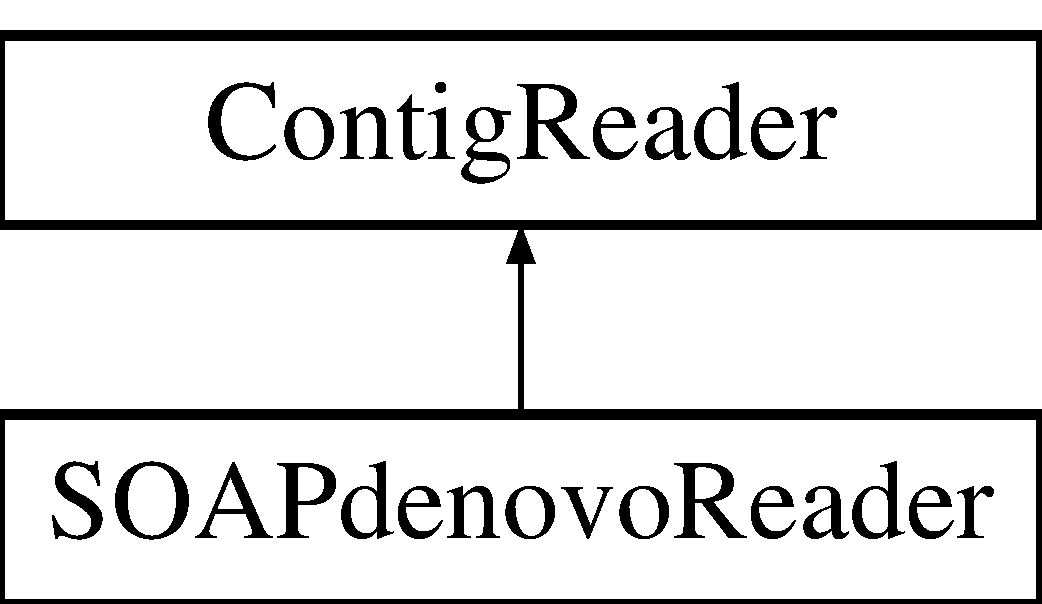
\includegraphics[height=2cm]{classSOAPdenovoReader}
\end{center}
\end{figure}
\subsection*{Public Member Functions}
\begin{DoxyCompactItemize}
\item 
\hyperlink{classSOAPdenovoReader_a29602e21bd8d8f21800eecbf13530331}{SOAPdenovoReader} ()
\item 
void \hyperlink{classSOAPdenovoReader_a308a9eb5c0b557c98705eaa4bd6626f7}{read} (const char $\ast$contigs\_\-file, \hyperlink{contig_8h_aa2acb8d3b78def617ec4509a1f684c4e}{ContigMap} $\ast$contigs)
\begin{DoxyCompactList}\small\item\em Reads contig information from SOAPdenovo contigs file. \item\end{DoxyCompactList}\end{DoxyCompactItemize}


\subsection{Detailed Description}
SOAPdenovo contigs file reader. Enables reading contig information from the output of \href{http://soap.genomics.org.cn/soapdenovo.html}{\tt SOAPdenovo} assembler. 

\subsection{Constructor \& Destructor Documentation}
\hypertarget{classSOAPdenovoReader_a29602e21bd8d8f21800eecbf13530331}{
\index{SOAPdenovoReader@{SOAPdenovoReader}!SOAPdenovoReader@{SOAPdenovoReader}}
\index{SOAPdenovoReader@{SOAPdenovoReader}!SOAPdenovoReader@{SOAPdenovoReader}}
\subsubsection[{SOAPdenovoReader}]{\setlength{\rightskip}{0pt plus 5cm}SOAPdenovoReader::SOAPdenovoReader ()}}
\label{classSOAPdenovoReader_a29602e21bd8d8f21800eecbf13530331}
An empty constructor. 

\subsection{Member Function Documentation}
\hypertarget{classSOAPdenovoReader_a308a9eb5c0b557c98705eaa4bd6626f7}{
\index{SOAPdenovoReader@{SOAPdenovoReader}!read@{read}}
\index{read@{read}!SOAPdenovoReader@{SOAPdenovoReader}}
\subsubsection[{read}]{\setlength{\rightskip}{0pt plus 5cm}void SOAPdenovoReader::read (const char $\ast$ {\em contigs\_\-file}, \/  {\bf ContigMap} $\ast$ {\em contigs})\hspace{0.3cm}{\ttfamily  \mbox{[}virtual\mbox{]}}}}
\label{classSOAPdenovoReader_a308a9eb5c0b557c98705eaa4bd6626f7}


Reads contig information from SOAPdenovo contigs file. 
\begin{DoxyParams}{Parameters}
\item[{\em contigs\_\-file}]path to contigs file \item[{\em contigs}]map with contig information \end{DoxyParams}
 

Implements \hyperlink{classContigReader_a935b5918388b7009b36e639391cfa4e8}{ContigReader}.

The documentation for this class was generated from the following files:\begin{DoxyCompactItemize}
\item 
/mnt/ScratchPool/bertrandd/OPERA\_\-MS/OperaMS2.0/SIGMA++/1.4/\hyperlink{contig__reader_8h}{contig\_\-reader.h}\item 
/mnt/ScratchPool/bertrandd/OPERA\_\-MS/OperaMS2.0/SIGMA++/1.4/\hyperlink{contig__reader_8cpp}{contig\_\-reader.cpp}\end{DoxyCompactItemize}

\hypertarget{classVelvetReader}{
\section{VelvetReader Class Reference}
\label{classVelvetReader}\index{VelvetReader@{VelvetReader}}
}


Velvet contigs file reader.  


{\ttfamily \#include $<$/mnt/ScratchPool/bertrandd/OPERA\_\-MS/OperaMS2.0/SIGMA++/1.4/contig\_\-reader.h$>$}Inheritance diagram for VelvetReader::\begin{figure}[H]
\begin{center}
\leavevmode
\includegraphics[height=2cm]{classVelvetReader}
\end{center}
\end{figure}
\subsection*{Public Member Functions}
\begin{DoxyCompactItemize}
\item 
\hyperlink{classVelvetReader_a94428db9b6e554a49a4cb22fd5ceec7a}{VelvetReader} ()
\item 
void \hyperlink{classVelvetReader_a0121c85cb0fefcc3f0c52f134756ed2e}{read} (const char $\ast$contigs\_\-file, \hyperlink{contig_8h_aa2acb8d3b78def617ec4509a1f684c4e}{ContigMap} $\ast$contigs)
\begin{DoxyCompactList}\small\item\em Reads contig information from Velvet contigs file. \item\end{DoxyCompactList}\end{DoxyCompactItemize}


\subsection{Detailed Description}
Velvet contigs file reader. Enables reading contig information from the output of \href{https://www.ebi.ac.uk/~zerbino/velvet/}{\tt Velvet} assembler. 

\subsection{Constructor \& Destructor Documentation}
\hypertarget{classVelvetReader_a94428db9b6e554a49a4cb22fd5ceec7a}{
\index{VelvetReader@{VelvetReader}!VelvetReader@{VelvetReader}}
\index{VelvetReader@{VelvetReader}!VelvetReader@{VelvetReader}}
\subsubsection[{VelvetReader}]{\setlength{\rightskip}{0pt plus 5cm}VelvetReader::VelvetReader ()}}
\label{classVelvetReader_a94428db9b6e554a49a4cb22fd5ceec7a}
An empty constructor. 

\subsection{Member Function Documentation}
\hypertarget{classVelvetReader_a0121c85cb0fefcc3f0c52f134756ed2e}{
\index{VelvetReader@{VelvetReader}!read@{read}}
\index{read@{read}!VelvetReader@{VelvetReader}}
\subsubsection[{read}]{\setlength{\rightskip}{0pt plus 5cm}void VelvetReader::read (const char $\ast$ {\em contigs\_\-file}, \/  {\bf ContigMap} $\ast$ {\em contigs})\hspace{0.3cm}{\ttfamily  \mbox{[}virtual\mbox{]}}}}
\label{classVelvetReader_a0121c85cb0fefcc3f0c52f134756ed2e}


Reads contig information from Velvet contigs file. 
\begin{DoxyParams}{Parameters}
\item[{\em contigs\_\-file}]path to contigs file \item[{\em contigs}]map with contig information \end{DoxyParams}
 

Implements \hyperlink{classContigReader_a935b5918388b7009b36e639391cfa4e8}{ContigReader}.

The documentation for this class was generated from the following files:\begin{DoxyCompactItemize}
\item 
/mnt/ScratchPool/bertrandd/OPERA\_\-MS/OperaMS2.0/SIGMA++/1.4/\hyperlink{contig__reader_8h}{contig\_\-reader.h}\item 
/mnt/ScratchPool/bertrandd/OPERA\_\-MS/OperaMS2.0/SIGMA++/1.4/\hyperlink{contig__reader_8cpp}{contig\_\-reader.cpp}\end{DoxyCompactItemize}

\chapter{File Documentation}
\hypertarget{cluster_8cpp}{
\section{/mnt/ScratchPool/bertrandd/OPERA\_\-MS/OperaMS2.0/SIGMA++/1.4/cluster.cpp File Reference}
\label{cluster_8cpp}\index{/mnt/ScratchPool/bertrandd/OPERA\_\-MS/OperaMS2.0/SIGMA++/1.4/cluster.cpp@{/mnt/ScratchPool/bertrandd/OPERA\_\-MS/OperaMS2.0/SIGMA++/1.4/cluster.cpp}}
}
{\ttfamily \#include $<$cstdlib$>$}\par
{\ttfamily \#include \char`\"{}cluster.h\char`\"{}}\par
{\ttfamily \#include \char`\"{}sigma.h\char`\"{}}\par

\hypertarget{cluster_8h}{
\section{/mnt/ScratchPool/bertrandd/OPERA\_\-MS/OperaMS2.0/SIGMA++/1.4/cluster.h File Reference}
\label{cluster_8h}\index{/mnt/ScratchPool/bertrandd/OPERA\_\-MS/OperaMS2.0/SIGMA++/1.4/cluster.h@{/mnt/ScratchPool/bertrandd/OPERA\_\-MS/OperaMS2.0/SIGMA++/1.4/cluster.h}}
}
{\ttfamily \#include $<$stack$>$}\par
{\ttfamily \#include $<$unordered\_\-set$>$}\par
{\ttfamily \#include \char`\"{}contig.h\char`\"{}}\par
\subsection*{Classes}
\begin{DoxyCompactItemize}
\item 
class \hyperlink{classCluster}{Cluster}
\begin{DoxyCompactList}\small\item\em A class for representing clusters in hierarchical clustering trees. \item\end{DoxyCompactList}\end{DoxyCompactItemize}
\subsection*{Typedefs}
\begin{DoxyCompactItemize}
\item 
typedef std::stack$<$ \hyperlink{classCluster}{Cluster} $\ast$ $>$ \hyperlink{cluster_8h_acc407f009938702d98b9f142f69f02a9}{ClusterStack}
\item 
typedef std::unordered\_\-set$<$ \hyperlink{classCluster}{Cluster} $\ast$ $>$ \hyperlink{cluster_8h_ac282f47ef6416737ea8a6f13a61bfd86}{ClusterSet}
\end{DoxyCompactItemize}


\subsection{Typedef Documentation}
\hypertarget{cluster_8h_ac282f47ef6416737ea8a6f13a61bfd86}{
\index{cluster.h@{cluster.h}!ClusterSet@{ClusterSet}}
\index{ClusterSet@{ClusterSet}!cluster.h@{cluster.h}}
\subsubsection[{ClusterSet}]{\setlength{\rightskip}{0pt plus 5cm}typedef std::unordered\_\-set$<${\bf Cluster}$\ast$$>$ {\bf ClusterSet}}}
\label{cluster_8h_ac282f47ef6416737ea8a6f13a61bfd86}
A set of clusters used for storing current roots of hierarchical clustering trees. \hypertarget{cluster_8h_acc407f009938702d98b9f142f69f02a9}{
\index{cluster.h@{cluster.h}!ClusterStack@{ClusterStack}}
\index{ClusterStack@{ClusterStack}!cluster.h@{cluster.h}}
\subsubsection[{ClusterStack}]{\setlength{\rightskip}{0pt plus 5cm}typedef std::stack$<${\bf Cluster}$\ast$$>$ {\bf ClusterStack}}}
\label{cluster_8h_acc407f009938702d98b9f142f69f02a9}
A stack of clusters used for recursive operations on hierarchical clustering trees. 
\hypertarget{cluster__graph_8cpp}{
\section{/mnt/ScratchPool/bertrandd/OPERA\_\-MS/OperaMS2.0/SIGMA++/1.4/cluster\_\-graph.cpp File Reference}
\label{cluster__graph_8cpp}\index{/mnt/ScratchPool/bertrandd/OPERA\_\-MS/OperaMS2.0/SIGMA++/1.4/cluster\_\-graph.cpp@{/mnt/ScratchPool/bertrandd/OPERA\_\-MS/OperaMS2.0/SIGMA++/1.4/cluster\_\-graph.cpp}}
}
{\ttfamily \#include $<$cstdlib$>$}\par
{\ttfamily \#include $<$cstdio$>$}\par
{\ttfamily \#include $<$cmath$>$}\par
{\ttfamily \#include \char`\"{}cluster\_\-graph.h\char`\"{}}\par
{\ttfamily \#include \char`\"{}sigma.h\char`\"{}}\par

\hypertarget{cluster__graph_8h}{
\section{/mnt/ScratchPool/bertrandd/OPERA\_\-MS/OperaMS2.0/SIGMA++/1.4/cluster\_\-graph.h File Reference}
\label{cluster__graph_8h}\index{/mnt/ScratchPool/bertrandd/OPERA\_\-MS/OperaMS2.0/SIGMA++/1.4/cluster\_\-graph.h@{/mnt/ScratchPool/bertrandd/OPERA\_\-MS/OperaMS2.0/SIGMA++/1.4/cluster\_\-graph.h}}
}
{\ttfamily \#include \char`\"{}contig.h\char`\"{}}\par
{\ttfamily \#include \char`\"{}edge.h\char`\"{}}\par
{\ttfamily \#include \char`\"{}cluster.h\char`\"{}}\par
{\ttfamily \#include \char`\"{}probability\_\-distribution.h\char`\"{}}\par
\subsection*{Classes}
\begin{DoxyCompactItemize}
\item 
class \hyperlink{classClusterGraph}{ClusterGraph}
\begin{DoxyCompactList}\small\item\em A class for representing a graph of hierarchical clustering trees. \item\end{DoxyCompactList}\end{DoxyCompactItemize}

\hypertarget{contig_8cpp}{
\section{/mnt/ScratchPool/bertrandd/OPERA\_\-MS/OperaMS2.0/SIGMA++/1.4/contig.cpp File Reference}
\label{contig_8cpp}\index{/mnt/ScratchPool/bertrandd/OPERA\_\-MS/OperaMS2.0/SIGMA++/1.4/contig.cpp@{/mnt/ScratchPool/bertrandd/OPERA\_\-MS/OperaMS2.0/SIGMA++/1.4/contig.cpp}}
}
{\ttfamily \#include $<$cstdlib$>$}\par
{\ttfamily \#include $<$algorithm$>$}\par
{\ttfamily \#include $<$vector$>$}\par
{\ttfamily \#include \char`\"{}contig.h\char`\"{}}\par
{\ttfamily \#include \char`\"{}sigma.h\char`\"{}}\par
\subsection*{Functions}
\begin{DoxyCompactItemize}
\item 
double \hyperlink{contig_8cpp_aa1c99e9f30b09d463aeea0036cd27181}{compute\_\-vmr} (\hyperlink{contig_8h_aa2acb8d3b78def617ec4509a1f684c4e}{ContigMap} $\ast$contigs)
\begin{DoxyCompactList}\small\item\em Computes a global read count variance-\/to-\/mean ratio on contig windows. \item\end{DoxyCompactList}\end{DoxyCompactItemize}


\subsection{Function Documentation}
\hypertarget{contig_8cpp_aa1c99e9f30b09d463aeea0036cd27181}{
\index{contig.cpp@{contig.cpp}!compute\_\-vmr@{compute\_\-vmr}}
\index{compute\_\-vmr@{compute\_\-vmr}!contig.cpp@{contig.cpp}}
\subsubsection[{compute\_\-vmr}]{\setlength{\rightskip}{0pt plus 5cm}double compute\_\-vmr ({\bf ContigMap} $\ast$ {\em contigs})}}
\label{contig_8cpp_aa1c99e9f30b09d463aeea0036cd27181}


Computes a global read count variance-\/to-\/mean ratio on contig windows. 
\begin{DoxyParams}{Parameters}
\item[{\em contigs}]map with contig information \end{DoxyParams}
\begin{DoxyReturn}{Returns}
read count variance-\/to-\/mean ratio on contig windows 
\end{DoxyReturn}

\hypertarget{contig_8h}{
\section{/mnt/ScratchPool/bertrandd/OPERA\_\-MS/OperaMS2.0/SIGMA++/1.4/contig.h File Reference}
\label{contig_8h}\index{/mnt/ScratchPool/bertrandd/OPERA\_\-MS/OperaMS2.0/SIGMA++/1.4/contig.h@{/mnt/ScratchPool/bertrandd/OPERA\_\-MS/OperaMS2.0/SIGMA++/1.4/contig.h}}
}
{\ttfamily \#include $<$string$>$}\par
{\ttfamily \#include $<$unordered\_\-map$>$}\par
\subsection*{Classes}
\begin{DoxyCompactItemize}
\item 
class \hyperlink{classContig}{Contig}
\begin{DoxyCompactList}\small\item\em A class for representing contigs in the assembly graph. \item\end{DoxyCompactList}\item 
class \hyperlink{classContigIO}{ContigIO}
\begin{DoxyCompactList}\small\item\em Class containing internal contigs IO functions. \item\end{DoxyCompactList}\end{DoxyCompactItemize}
\subsection*{Typedefs}
\begin{DoxyCompactItemize}
\item 
typedef std::unordered\_\-map$<$ std::string, \hyperlink{classContig}{Contig} $\ast$ $>$ \hyperlink{contig_8h_aa2acb8d3b78def617ec4509a1f684c4e}{ContigMap}
\end{DoxyCompactItemize}
\subsection*{Functions}
\begin{DoxyCompactItemize}
\item 
double \hyperlink{contig_8h_aa1c99e9f30b09d463aeea0036cd27181}{compute\_\-vmr} (\hyperlink{contig_8h_aa2acb8d3b78def617ec4509a1f684c4e}{ContigMap} $\ast$contigs)
\begin{DoxyCompactList}\small\item\em Computes a global read count variance-\/to-\/mean ratio on contig windows. \item\end{DoxyCompactList}\end{DoxyCompactItemize}


\subsection{Typedef Documentation}
\hypertarget{contig_8h_aa2acb8d3b78def617ec4509a1f684c4e}{
\index{contig.h@{contig.h}!ContigMap@{ContigMap}}
\index{ContigMap@{ContigMap}!contig.h@{contig.h}}
\subsubsection[{ContigMap}]{\setlength{\rightskip}{0pt plus 5cm}typedef std::unordered\_\-map$<$std::string, {\bf Contig}$\ast$$>$ {\bf ContigMap}}}
\label{contig_8h_aa2acb8d3b78def617ec4509a1f684c4e}
A map with contig ids as keys and pointers to corresponding objects as values. 

\subsection{Function Documentation}
\hypertarget{contig_8h_aa1c99e9f30b09d463aeea0036cd27181}{
\index{contig.h@{contig.h}!compute\_\-vmr@{compute\_\-vmr}}
\index{compute\_\-vmr@{compute\_\-vmr}!contig.h@{contig.h}}
\subsubsection[{compute\_\-vmr}]{\setlength{\rightskip}{0pt plus 5cm}double compute\_\-vmr ({\bf ContigMap} $\ast$ {\em contigs})}}
\label{contig_8h_aa1c99e9f30b09d463aeea0036cd27181}


Computes a global read count variance-\/to-\/mean ratio on contig windows. 
\begin{DoxyParams}{Parameters}
\item[{\em contigs}]map with contig information \end{DoxyParams}
\begin{DoxyReturn}{Returns}
read count variance-\/to-\/mean ratio on contig windows 
\end{DoxyReturn}

\hypertarget{contig__reader_8cpp}{
\section{/mnt/ScratchPool/bertrandd/OPERA\_\-MS/OperaMS2.0/SIGMA++/1.4/contig\_\-reader.cpp File Reference}
\label{contig__reader_8cpp}\index{/mnt/ScratchPool/bertrandd/OPERA\_\-MS/OperaMS2.0/SIGMA++/1.4/contig\_\-reader.cpp@{/mnt/ScratchPool/bertrandd/OPERA\_\-MS/OperaMS2.0/SIGMA++/1.4/contig\_\-reader.cpp}}
}
{\ttfamily \#include $<$cstdlib$>$}\par
{\ttfamily \#include $<$cstdio$>$}\par
{\ttfamily \#include \char`\"{}contig\_\-reader.h\char`\"{}}\par
{\ttfamily \#include \char`\"{}sigma.h\char`\"{}}\par

\hypertarget{contig__reader_8h}{
\section{/mnt/ScratchPool/bertrandd/OPERA\_\-MS/OperaMS2.0/SIGMA++/1.4/contig\_\-reader.h File Reference}
\label{contig__reader_8h}\index{/mnt/ScratchPool/bertrandd/OPERA\_\-MS/OperaMS2.0/SIGMA++/1.4/contig\_\-reader.h@{/mnt/ScratchPool/bertrandd/OPERA\_\-MS/OperaMS2.0/SIGMA++/1.4/contig\_\-reader.h}}
}
{\ttfamily \#include \char`\"{}contig.h\char`\"{}}\par
\subsection*{Classes}
\begin{DoxyCompactItemize}
\item 
class \hyperlink{classContigReader}{ContigReader}
\begin{DoxyCompactList}\small\item\em An interface for contigs file readers. \item\end{DoxyCompactList}\item 
class \hyperlink{classSOAPdenovoReader}{SOAPdenovoReader}
\begin{DoxyCompactList}\small\item\em SOAPdenovo contigs file reader. \item\end{DoxyCompactList}\item 
class \hyperlink{classVelvetReader}{VelvetReader}
\begin{DoxyCompactList}\small\item\em Velvet contigs file reader. \item\end{DoxyCompactList}\end{DoxyCompactItemize}

\hypertarget{edge_8cpp}{
\section{/mnt/ScratchPool/bertrandd/OPERA\_\-MS/OperaMS2.0/SIGMA++/1.4/edge.cpp File Reference}
\label{edge_8cpp}\index{/mnt/ScratchPool/bertrandd/OPERA\_\-MS/OperaMS2.0/SIGMA++/1.4/edge.cpp@{/mnt/ScratchPool/bertrandd/OPERA\_\-MS/OperaMS2.0/SIGMA++/1.4/edge.cpp}}
}
{\ttfamily \#include $<$cstdlib$>$}\par
{\ttfamily \#include \char`\"{}edge.h\char`\"{}}\par
{\ttfamily \#include \char`\"{}sigma.h\char`\"{}}\par
\subsection*{Functions}
\begin{DoxyCompactItemize}
\item 
bool \hyperlink{edge_8cpp_a49b989380f52aa039eca454b851cfe88}{operator==} (const \hyperlink{classEdge}{Edge} \&edge1, const \hyperlink{classEdge}{Edge} \&edge2)
\end{DoxyCompactItemize}


\subsection{Function Documentation}
\hypertarget{edge_8cpp_a49b989380f52aa039eca454b851cfe88}{
\index{edge.cpp@{edge.cpp}!operator==@{operator==}}
\index{operator==@{operator==}!edge.cpp@{edge.cpp}}
\subsubsection[{operator==}]{\setlength{\rightskip}{0pt plus 5cm}bool operator== (const {\bf Edge} \& {\em edge1}, \/  const {\bf Edge} \& {\em edge2})}}
\label{edge_8cpp_a49b989380f52aa039eca454b851cfe88}

\hypertarget{edge_8h}{
\section{/mnt/ScratchPool/bertrandd/OPERA\_\-MS/OperaMS2.0/SIGMA++/1.4/edge.h File Reference}
\label{edge_8h}\index{/mnt/ScratchPool/bertrandd/OPERA\_\-MS/OperaMS2.0/SIGMA++/1.4/edge.h@{/mnt/ScratchPool/bertrandd/OPERA\_\-MS/OperaMS2.0/SIGMA++/1.4/edge.h}}
}
{\ttfamily \#include $<$vector$>$}\par
{\ttfamily \#include $<$queue$>$}\par
{\ttfamily \#include $<$unordered\_\-set$>$}\par
{\ttfamily \#include $<$functional$>$}\par
{\ttfamily \#include \char`\"{}contig.h\char`\"{}}\par
\subsection*{Classes}
\begin{DoxyCompactItemize}
\item 
class \hyperlink{classEdge}{Edge}
\begin{DoxyCompactList}\small\item\em A class for representing scaffold edges in the assembly graph. \item\end{DoxyCompactList}\item 
class \hyperlink{classEdgeComparator}{EdgeComparator}
\begin{DoxyCompactList}\small\item\em Function object class for less-\/than inequality comparison of \hyperlink{classEdge}{Edge} objects. \item\end{DoxyCompactList}\item 
class \hyperlink{classEdgeHash}{EdgeHash}
\begin{DoxyCompactList}\small\item\em Function object class for computing hash values for \hyperlink{classEdge}{Edge} objects. \item\end{DoxyCompactList}\end{DoxyCompactItemize}
\subsection*{Typedefs}
\begin{DoxyCompactItemize}
\item 
typedef std::unordered\_\-set$<$ \hyperlink{classEdge}{Edge}, \hyperlink{classEdgeHash}{EdgeHash} $>$ \hyperlink{edge_8h_ad07b5df6e7cfe15cad88e3b25d48c84f}{EdgeSet}
\item 
typedef std::priority\_\-queue$<$ \hyperlink{classEdge}{Edge}, std::vector$<$ \hyperlink{classEdge}{Edge} $>$, \hyperlink{classEdgeComparator}{EdgeComparator} $>$ \hyperlink{edge_8h_ada6d1f0d2fed8c49bc8ba085b524d726}{EdgeQueue}
\end{DoxyCompactItemize}


\subsection{Typedef Documentation}
\hypertarget{edge_8h_ada6d1f0d2fed8c49bc8ba085b524d726}{
\index{edge.h@{edge.h}!EdgeQueue@{EdgeQueue}}
\index{EdgeQueue@{EdgeQueue}!edge.h@{edge.h}}
\subsubsection[{EdgeQueue}]{\setlength{\rightskip}{0pt plus 5cm}typedef std::priority\_\-queue$<${\bf Edge}, std::vector$<${\bf Edge}$>$, {\bf EdgeComparator}$>$ {\bf EdgeQueue}}}
\label{edge_8h_ada6d1f0d2fed8c49bc8ba085b524d726}
A priority queue of edges used for building clustering trees. \hypertarget{edge_8h_ad07b5df6e7cfe15cad88e3b25d48c84f}{
\index{edge.h@{edge.h}!EdgeSet@{EdgeSet}}
\index{EdgeSet@{EdgeSet}!edge.h@{edge.h}}
\subsubsection[{EdgeSet}]{\setlength{\rightskip}{0pt plus 5cm}typedef std::unordered\_\-set$<${\bf Edge}, {\bf EdgeHash}$>$ {\bf EdgeSet}}}
\label{edge_8h_ad07b5df6e7cfe15cad88e3b25d48c84f}
A hash set of edges used for storing unique edges when reading edges files. 
\hypertarget{edge__reader_8cpp}{
\section{/mnt/ScratchPool/bertrandd/OPERA\_\-MS/OperaMS2.0/SIGMA++/1.4/edge\_\-reader.cpp File Reference}
\label{edge__reader_8cpp}\index{/mnt/ScratchPool/bertrandd/OPERA\_\-MS/OperaMS2.0/SIGMA++/1.4/edge\_\-reader.cpp@{/mnt/ScratchPool/bertrandd/OPERA\_\-MS/OperaMS2.0/SIGMA++/1.4/edge\_\-reader.cpp}}
}
{\ttfamily \#include $<$cstdlib$>$}\par
{\ttfamily \#include $<$cstdio$>$}\par
{\ttfamily \#include \char`\"{}edge\_\-reader.h\char`\"{}}\par
{\ttfamily \#include \char`\"{}sigma.h\char`\"{}}\par

\hypertarget{edge__reader_8h}{
\section{/mnt/ScratchPool/bertrandd/OPERA\_\-MS/OperaMS2.0/SIGMA++/1.4/edge\_\-reader.h File Reference}
\label{edge__reader_8h}\index{/mnt/ScratchPool/bertrandd/OPERA\_\-MS/OperaMS2.0/SIGMA++/1.4/edge\_\-reader.h@{/mnt/ScratchPool/bertrandd/OPERA\_\-MS/OperaMS2.0/SIGMA++/1.4/edge\_\-reader.h}}
}
{\ttfamily \#include \char`\"{}contig.h\char`\"{}}\par
{\ttfamily \#include \char`\"{}edge.h\char`\"{}}\par
\subsection*{Classes}
\begin{DoxyCompactItemize}
\item 
class \hyperlink{classEdgeReader}{EdgeReader}
\begin{DoxyCompactList}\small\item\em An interface for edges file readers. \item\end{DoxyCompactList}\item 
class \hyperlink{classOperaBundleReader}{OperaBundleReader}
\begin{DoxyCompactList}\small\item\em Opera edges file reader. \item\end{DoxyCompactList}\end{DoxyCompactItemize}

\hypertarget{mapping__reader_8cpp}{
\section{/mnt/ScratchPool/bertrandd/OPERA\_\-MS/OperaMS2.0/SIGMA++/1.4/mapping\_\-reader.cpp File Reference}
\label{mapping__reader_8cpp}\index{/mnt/ScratchPool/bertrandd/OPERA\_\-MS/OperaMS2.0/SIGMA++/1.4/mapping\_\-reader.cpp@{/mnt/ScratchPool/bertrandd/OPERA\_\-MS/OperaMS2.0/SIGMA++/1.4/mapping\_\-reader.cpp}}
}
{\ttfamily \#include $<$cstdlib$>$}\par
{\ttfamily \#include $<$cstdio$>$}\par
{\ttfamily \#include \char`\"{}mapping\_\-reader.h\char`\"{}}\par
{\ttfamily \#include \char`\"{}sigma.h\char`\"{}}\par

\hypertarget{mapping__reader_8h}{
\section{/mnt/ScratchPool/bertrandd/OPERA\_\-MS/OperaMS2.0/SIGMA++/1.4/mapping\_\-reader.h File Reference}
\label{mapping__reader_8h}\index{/mnt/ScratchPool/bertrandd/OPERA\_\-MS/OperaMS2.0/SIGMA++/1.4/mapping\_\-reader.h@{/mnt/ScratchPool/bertrandd/OPERA\_\-MS/OperaMS2.0/SIGMA++/1.4/mapping\_\-reader.h}}
}
{\ttfamily \#include \char`\"{}contig.h\char`\"{}}\par
\subsection*{Classes}
\begin{DoxyCompactItemize}
\item 
class \hyperlink{classMappingReader}{MappingReader}
\begin{DoxyCompactList}\small\item\em An interface for mapping file readers. \item\end{DoxyCompactList}\item 
class \hyperlink{classSAMReader}{SAMReader}
\begin{DoxyCompactList}\small\item\em SAM mapping file reader. \item\end{DoxyCompactList}\end{DoxyCompactItemize}

\hypertarget{probability__distribution_8cpp}{
\section{/mnt/ScratchPool/bertrandd/OPERA\_\-MS/OperaMS2.0/SIGMA++/1.4/probability\_\-distribution.cpp File Reference}
\label{probability__distribution_8cpp}\index{/mnt/ScratchPool/bertrandd/OPERA\_\-MS/OperaMS2.0/SIGMA++/1.4/probability\_\-distribution.cpp@{/mnt/ScratchPool/bertrandd/OPERA\_\-MS/OperaMS2.0/SIGMA++/1.4/probability\_\-distribution.cpp}}
}
{\ttfamily \#include $<$cstdlib$>$}\par
{\ttfamily \#include $<$cmath$>$}\par
{\ttfamily \#include \char`\"{}probability\_\-distribution.h\char`\"{}}\par
\subsection*{Functions}
\begin{DoxyCompactItemize}
\item 
static double \hyperlink{probability__distribution_8cpp_aa008ab82cd1e3a7c734abbccfdf47d25}{stirling\_\-log\_\-factorial} (double x)
\begin{DoxyCompactList}\small\item\em Computes Stirling's series approximation of log(x!). \item\end{DoxyCompactList}\end{DoxyCompactItemize}
\subsection*{Variables}
\begin{Indent}{\bf }\par
{\em \label{_amgrpd41d8cd98f00b204e9800998ecf8427e}
 }\begin{DoxyCompactItemize}
\item 
static const double \hyperlink{probability__distribution_8cpp_abb30260352ac2c99c17ad6ba1b9eec95}{LOG\_\-SQRT2PI} = 0.5 $\ast$ log(2.0 $\ast$ 3.14159265358979323846)
\item 
static const double \hyperlink{probability__distribution_8cpp_a281748e1c9170c319467b964e00ffdcd}{LC1} = 1.0 / 12.0
\item 
static const double \hyperlink{probability__distribution_8cpp_ad40081cd1b03fabc256d282bc182600c}{LC2} = -\/1.0 / 360.0
\item 
static const double \hyperlink{probability__distribution_8cpp_a051c91b0471cbae85672657b5784240b}{LC3} = 1.0 / 1260.0
\item 
static const double \hyperlink{probability__distribution_8cpp_add3817a2ccf5bb9c63838889236f4a5e}{LC4} = -\/1.0 / 1680.0
\end{DoxyCompactItemize}
\end{Indent}


\subsection{Function Documentation}
\hypertarget{probability__distribution_8cpp_aa008ab82cd1e3a7c734abbccfdf47d25}{
\index{probability\_\-distribution.cpp@{probability\_\-distribution.cpp}!stirling\_\-log\_\-factorial@{stirling\_\-log\_\-factorial}}
\index{stirling\_\-log\_\-factorial@{stirling\_\-log\_\-factorial}!probability_distribution.cpp@{probability\_\-distribution.cpp}}
\subsubsection[{stirling\_\-log\_\-factorial}]{\setlength{\rightskip}{0pt plus 5cm}static double stirling\_\-log\_\-factorial (double {\em x})\hspace{0.3cm}{\ttfamily  \mbox{[}inline, static\mbox{]}}}}
\label{probability__distribution_8cpp_aa008ab82cd1e3a7c734abbccfdf47d25}


Computes Stirling's series approximation of log(x!). Computes \href{http://en.wikipedia.org/wiki/Stirling%27s_approximation>}{\tt Stirling's series approximation} of log(x!) using log(x!) = log(x) + log((x-\/1)!) = log(x) + log(gamma(x)).


\begin{DoxyParams}{Parameters}
\item[{\em x}]value for which the approximation is computed \end{DoxyParams}
\begin{DoxyReturn}{Returns}
Stirling's series approximation of log(x!) 
\end{DoxyReturn}


\subsection{Variable Documentation}
\hypertarget{probability__distribution_8cpp_a281748e1c9170c319467b964e00ffdcd}{
\index{probability\_\-distribution.cpp@{probability\_\-distribution.cpp}!LC1@{LC1}}
\index{LC1@{LC1}!probability_distribution.cpp@{probability\_\-distribution.cpp}}
\subsubsection[{LC1}]{\setlength{\rightskip}{0pt plus 5cm}const double {\bf LC1} = 1.0 / 12.0\hspace{0.3cm}{\ttfamily  \mbox{[}static\mbox{]}}}}
\label{probability__distribution_8cpp_a281748e1c9170c319467b964e00ffdcd}
Constant for Stirling's series approximation of log(x!). \hypertarget{probability__distribution_8cpp_ad40081cd1b03fabc256d282bc182600c}{
\index{probability\_\-distribution.cpp@{probability\_\-distribution.cpp}!LC2@{LC2}}
\index{LC2@{LC2}!probability_distribution.cpp@{probability\_\-distribution.cpp}}
\subsubsection[{LC2}]{\setlength{\rightskip}{0pt plus 5cm}const double {\bf LC2} = -\/1.0 / 360.0\hspace{0.3cm}{\ttfamily  \mbox{[}static\mbox{]}}}}
\label{probability__distribution_8cpp_ad40081cd1b03fabc256d282bc182600c}
Constant for Stirling's series approximation of log(x!). \hypertarget{probability__distribution_8cpp_a051c91b0471cbae85672657b5784240b}{
\index{probability\_\-distribution.cpp@{probability\_\-distribution.cpp}!LC3@{LC3}}
\index{LC3@{LC3}!probability_distribution.cpp@{probability\_\-distribution.cpp}}
\subsubsection[{LC3}]{\setlength{\rightskip}{0pt plus 5cm}const double {\bf LC3} = 1.0 / 1260.0\hspace{0.3cm}{\ttfamily  \mbox{[}static\mbox{]}}}}
\label{probability__distribution_8cpp_a051c91b0471cbae85672657b5784240b}
Constant for Stirling's series approximation of log(x!). \hypertarget{probability__distribution_8cpp_add3817a2ccf5bb9c63838889236f4a5e}{
\index{probability\_\-distribution.cpp@{probability\_\-distribution.cpp}!LC4@{LC4}}
\index{LC4@{LC4}!probability_distribution.cpp@{probability\_\-distribution.cpp}}
\subsubsection[{LC4}]{\setlength{\rightskip}{0pt plus 5cm}const double {\bf LC4} = -\/1.0 / 1680.0\hspace{0.3cm}{\ttfamily  \mbox{[}static\mbox{]}}}}
\label{probability__distribution_8cpp_add3817a2ccf5bb9c63838889236f4a5e}
Constant for Stirling's series approximation of log(x!). \hypertarget{probability__distribution_8cpp_abb30260352ac2c99c17ad6ba1b9eec95}{
\index{probability\_\-distribution.cpp@{probability\_\-distribution.cpp}!LOG\_\-SQRT2PI@{LOG\_\-SQRT2PI}}
\index{LOG\_\-SQRT2PI@{LOG\_\-SQRT2PI}!probability_distribution.cpp@{probability\_\-distribution.cpp}}
\subsubsection[{LOG\_\-SQRT2PI}]{\setlength{\rightskip}{0pt plus 5cm}const double {\bf LOG\_\-SQRT2PI} = 0.5 $\ast$ log(2.0 $\ast$ 3.14159265358979323846)\hspace{0.3cm}{\ttfamily  \mbox{[}static\mbox{]}}}}
\label{probability__distribution_8cpp_abb30260352ac2c99c17ad6ba1b9eec95}
Constant for Stirling's series approximation of log(x!). 
\hypertarget{probability__distribution_8h}{
\section{/mnt/ScratchPool/bertrandd/OPERA\_\-MS/OperaMS2.0/SIGMA++/1.4/probability\_\-distribution.h File Reference}
\label{probability__distribution_8h}\index{/mnt/ScratchPool/bertrandd/OPERA\_\-MS/OperaMS2.0/SIGMA++/1.4/probability\_\-distribution.h@{/mnt/ScratchPool/bertrandd/OPERA\_\-MS/OperaMS2.0/SIGMA++/1.4/probability\_\-distribution.h}}
}
\subsection*{Classes}
\begin{DoxyCompactItemize}
\item 
class \hyperlink{classProbabilityDistribution}{ProbabilityDistribution}
\begin{DoxyCompactList}\small\item\em An interface for probability distributions. \item\end{DoxyCompactList}\item 
class \hyperlink{classPoissonDistribution}{PoissonDistribution}
\begin{DoxyCompactList}\small\item\em An implementation of Poisson probability distribution. \item\end{DoxyCompactList}\item 
class \hyperlink{classNegativeBinomialDistribution}{NegativeBinomialDistribution}
\begin{DoxyCompactList}\small\item\em An implementation of negative binomial probability distribution. \item\end{DoxyCompactList}\end{DoxyCompactItemize}

\hypertarget{sigma_8cpp}{
\section{/mnt/ScratchPool/bertrandd/OPERA\_\-MS/OperaMS2.0/SIGMA++/1.4/sigma.cpp File Reference}
\label{sigma_8cpp}\index{/mnt/ScratchPool/bertrandd/OPERA\_\-MS/OperaMS2.0/SIGMA++/1.4/sigma.cpp@{/mnt/ScratchPool/bertrandd/OPERA\_\-MS/OperaMS2.0/SIGMA++/1.4/sigma.cpp}}
}
{\ttfamily \#include $<$cstdlib$>$}\par
{\ttfamily \#include $<$cstdio$>$}\par
{\ttfamily \#include $<$ctime$>$}\par
{\ttfamily \#include $<$iostream$>$}\par
{\ttfamily \#include $<$fstream$>$}\par
{\ttfamily \#include $<$sstream$>$}\par
{\ttfamily \#include \char`\"{}sigma.h\char`\"{}}\par
{\ttfamily \#include \char`\"{}contig\_\-reader.h\char`\"{}}\par
{\ttfamily \#include \char`\"{}mapping\_\-reader.h\char`\"{}}\par
{\ttfamily \#include \char`\"{}edge\_\-reader.h\char`\"{}}\par
{\ttfamily \#include \char`\"{}contig.h\char`\"{}}\par
{\ttfamily \#include \char`\"{}cluster.h\char`\"{}}\par
{\ttfamily \#include \char`\"{}cluster\_\-graph.h\char`\"{}}\par
{\ttfamily \#include \char`\"{}probability\_\-distribution.h\char`\"{}}\par
\subsection*{Functions}
\begin{DoxyCompactItemize}
\item 
int \hyperlink{sigma_8cpp_a3c04138a5bfe5d72780bb7e82a18e627}{main} (int argc, char $\ast$$\ast$argv)
\end{DoxyCompactItemize}


\subsection{Function Documentation}
\hypertarget{sigma_8cpp_a3c04138a5bfe5d72780bb7e82a18e627}{
\index{sigma.cpp@{sigma.cpp}!main@{main}}
\index{main@{main}!sigma.cpp@{sigma.cpp}}
\subsubsection[{main}]{\setlength{\rightskip}{0pt plus 5cm}int main (int {\em argc}, \/  char $\ast$$\ast$ {\em argv})}}
\label{sigma_8cpp_a3c04138a5bfe5d72780bb7e82a18e627}

\hypertarget{sigma_8h}{
\section{/mnt/ScratchPool/bertrandd/OPERA\_\-MS/OperaMS2.0/SIGMA++/1.4/sigma.h File Reference}
\label{sigma_8h}\index{/mnt/ScratchPool/bertrandd/OPERA\_\-MS/OperaMS2.0/SIGMA++/1.4/sigma.h@{/mnt/ScratchPool/bertrandd/OPERA\_\-MS/OperaMS2.0/SIGMA++/1.4/sigma.h}}
}
{\ttfamily \#include $<$string$>$}\par
{\ttfamily \#include $<$vector$>$}\par
{\ttfamily \#include $<$unordered\_\-map$>$}\par
\subsection*{Classes}
\begin{DoxyCompactItemize}
\item 
class \hyperlink{classSigma}{Sigma}
\begin{DoxyCompactList}\small\item\em Main configuration class. \item\end{DoxyCompactList}\end{DoxyCompactItemize}
\subsection*{Typedefs}
\begin{DoxyCompactItemize}
\item 
typedef std::unordered\_\-map$<$ std::string, std::string $>$ \hyperlink{sigma_8h_a731115adbc0862ff6c28d129591ab640}{ParamsMap}
\end{DoxyCompactItemize}


\subsection{Typedef Documentation}
\hypertarget{sigma_8h_a731115adbc0862ff6c28d129591ab640}{
\index{sigma.h@{sigma.h}!ParamsMap@{ParamsMap}}
\index{ParamsMap@{ParamsMap}!sigma.h@{sigma.h}}
\subsubsection[{ParamsMap}]{\setlength{\rightskip}{0pt plus 5cm}typedef std::unordered\_\-map$<$std::string, std::string$>$ {\bf ParamsMap}}}
\label{sigma_8h_a731115adbc0862ff6c28d129591ab640}
A map for storing key-\/value configuration parameters. 
\printindex
\end{document}
